\chapter{Procesamiento Digital de Señales}


\section{Sistemas discretos}
\begin{figure}[H]
\centering
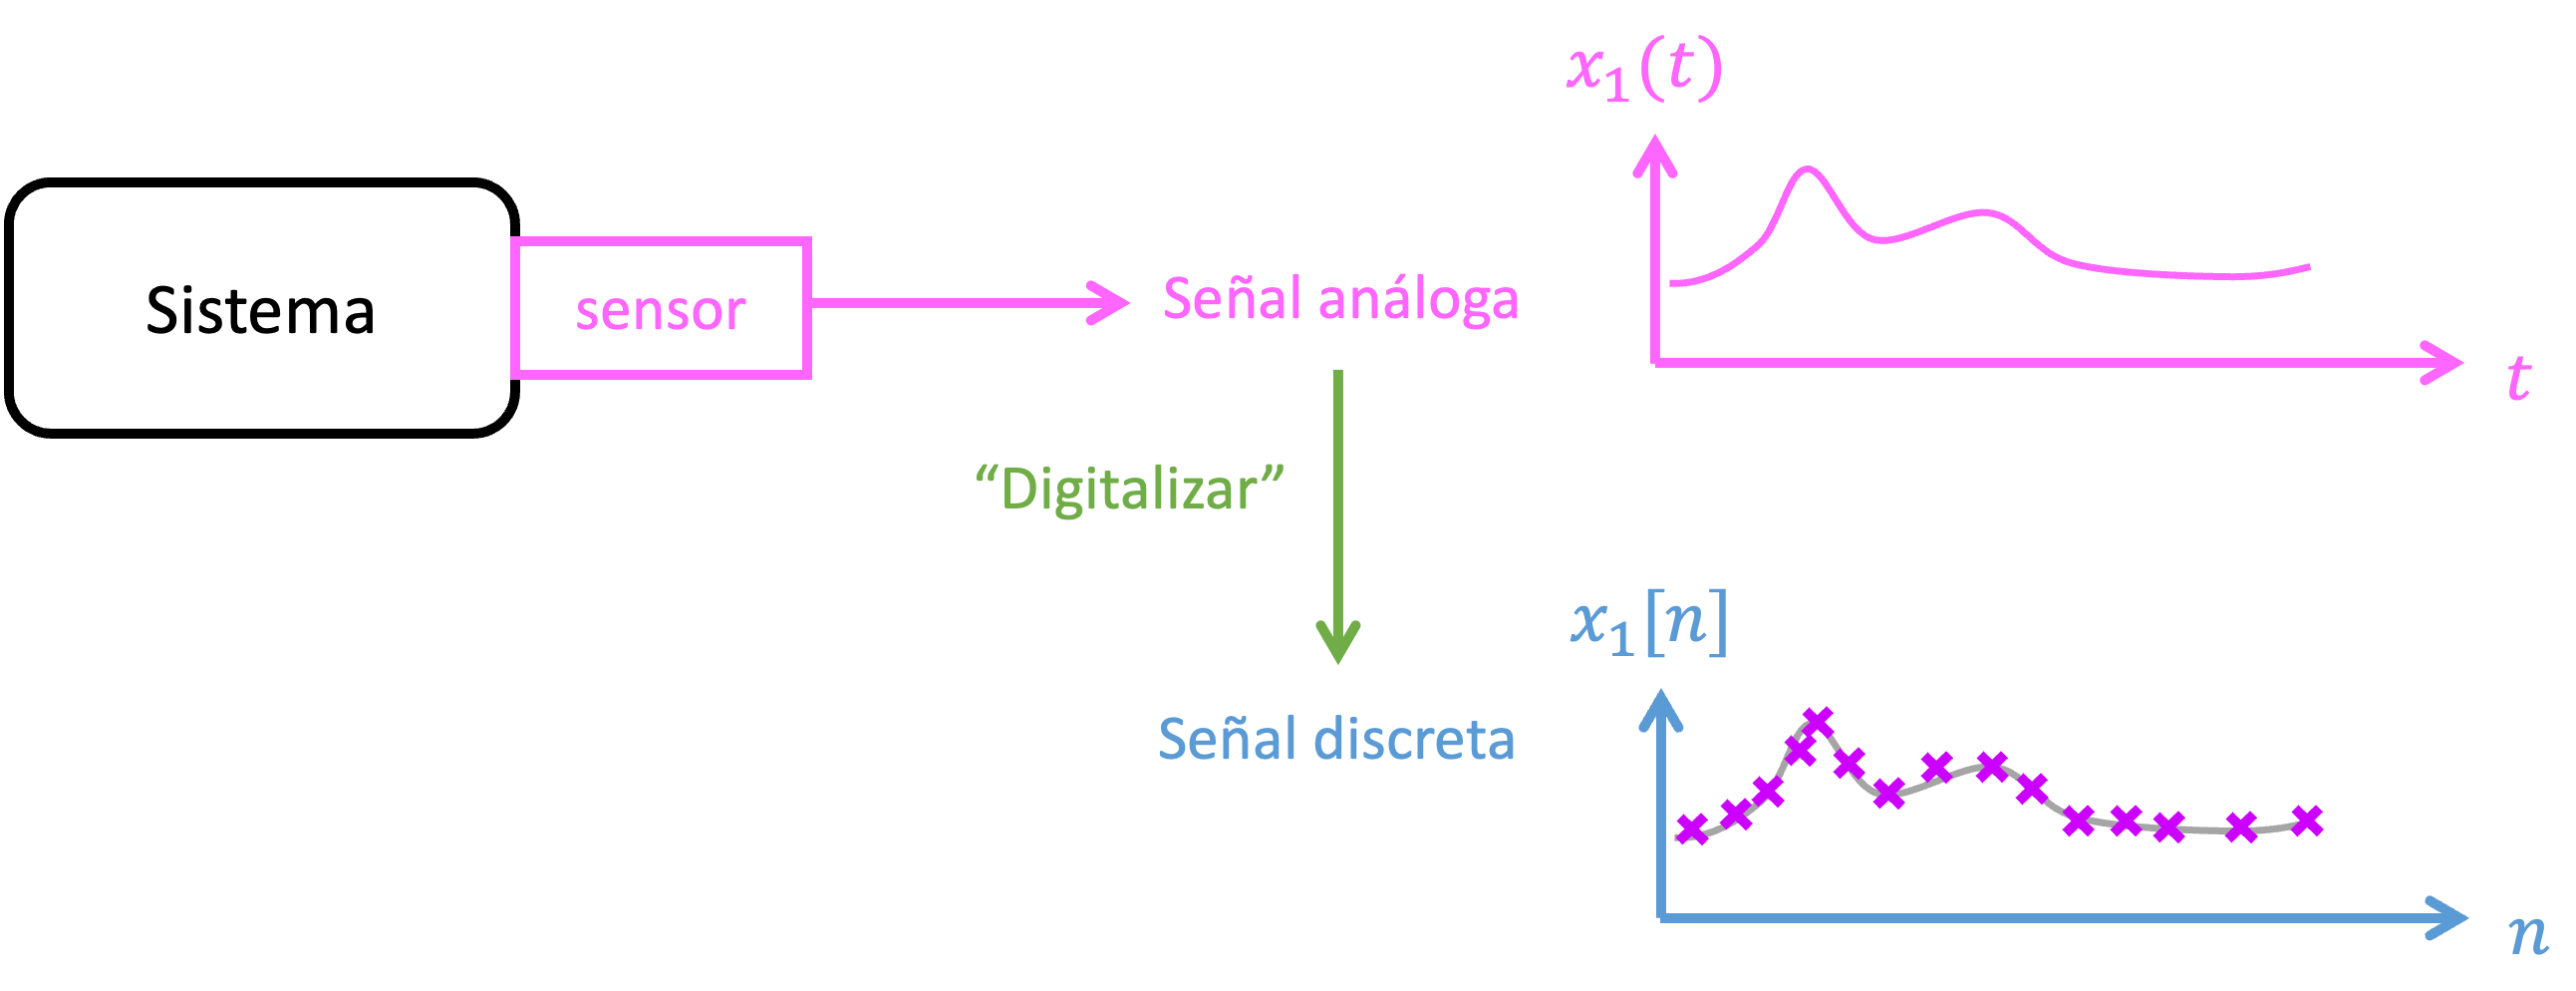
\includegraphics[scale=0.7]{Figuras/sist_discreto.png}
\end{figure}
\underline{Nota}: Computadores representan números utilizando dígitos binarios (bits, flip-flops). Es necesario convertir una señal análoga a discreta.\\

\par \underline{Muestreo (sampling)}: 
\begin{enumerate}
    \item Muestreo en el tiempo $\Longrightarrow$ Sampling
    \item Muestreo en amplitud $\Longrightarrow$ Quantization
\end{enumerate}

Máquina 16 bits $\Longrightarrow$ Números utilizando $2^{16}$ cifras significativas.
\begin{align*}
    \text{Bit} = \left\{ \begin{array}{l}
             0 \\
             1
             \end{array}
   \right. \Longrightarrow 65536 \text{ cifras significativas}
\end{align*}

\par \underline{Sistema discreto}:\\
\begin{figure}[H]
\centering
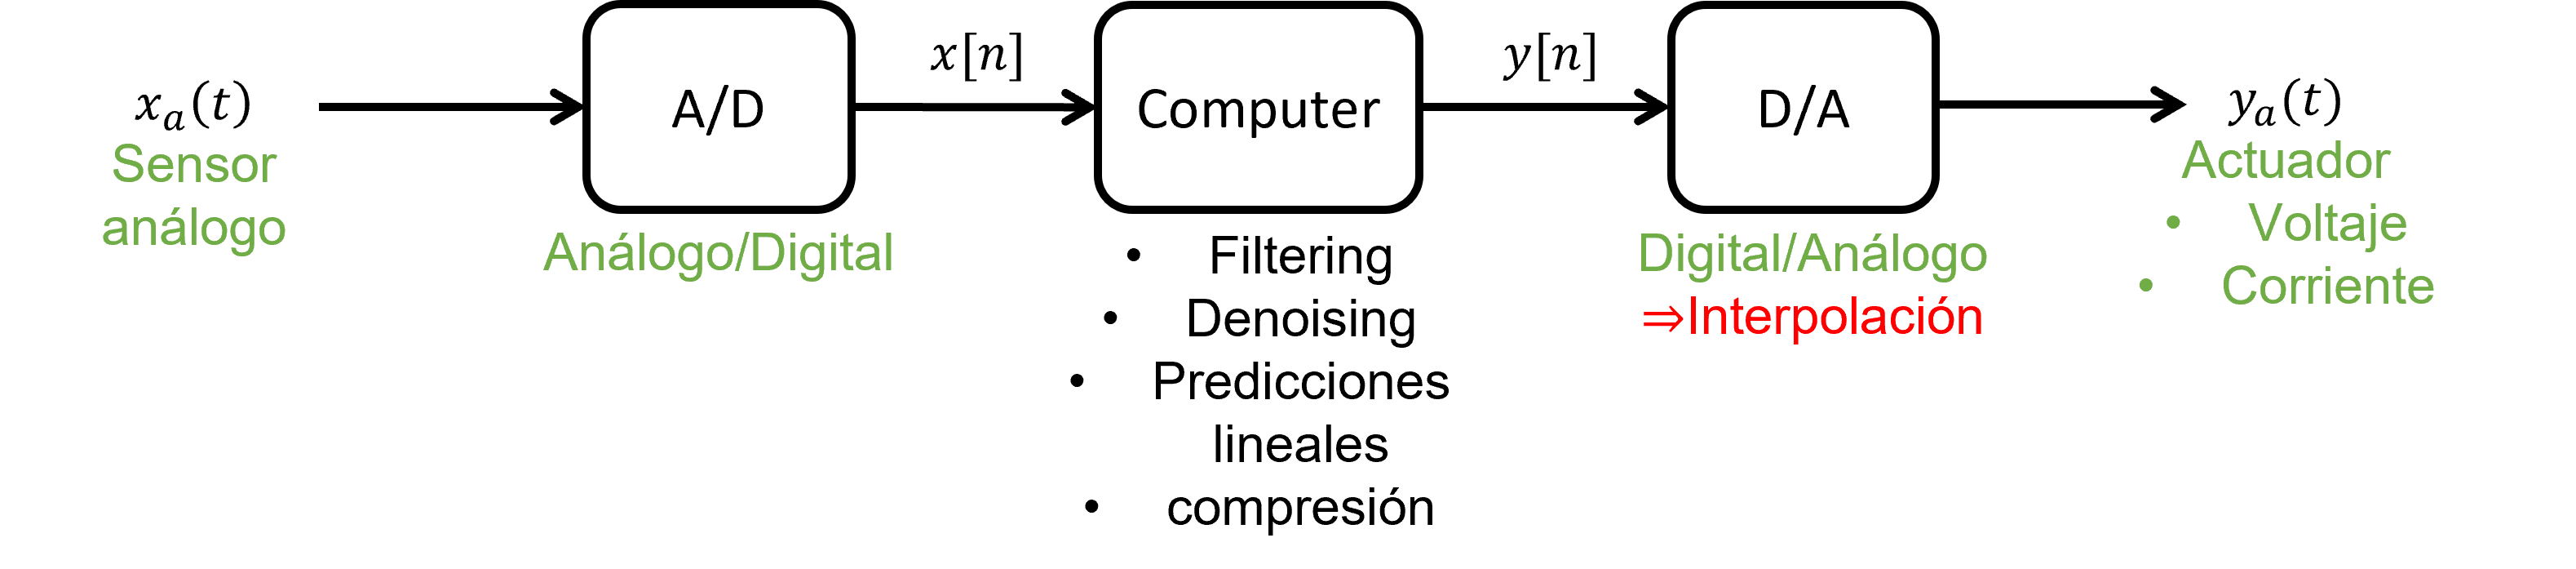
\includegraphics[scale=0.7]{Figuras/sistema_discret.png}
\end{figure}

$x[n]$: señal en tiempo discreto.\\
$$x[n]=x_a(nT)$$
T: intervalo de muestreo, n: índice (número entero)\\

\begin{figure}[H]
\centering
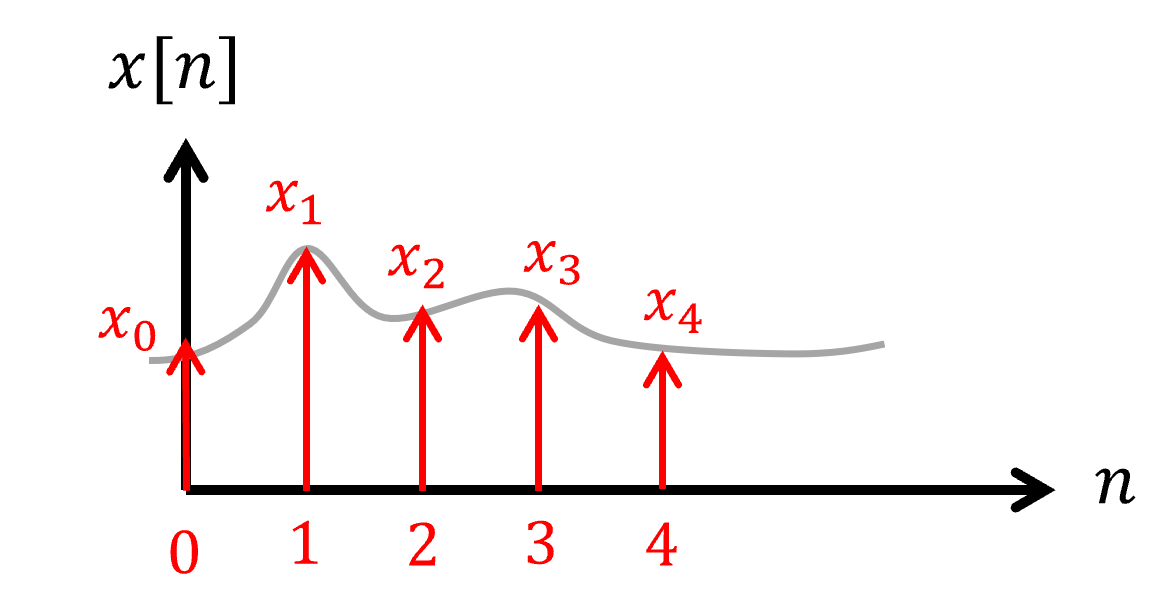
\includegraphics[scale=0.7]{Figuras/xn.png}
\end{figure}

\par \underline{Función pulso unitario}:
\begin{figure}[H]
\centering
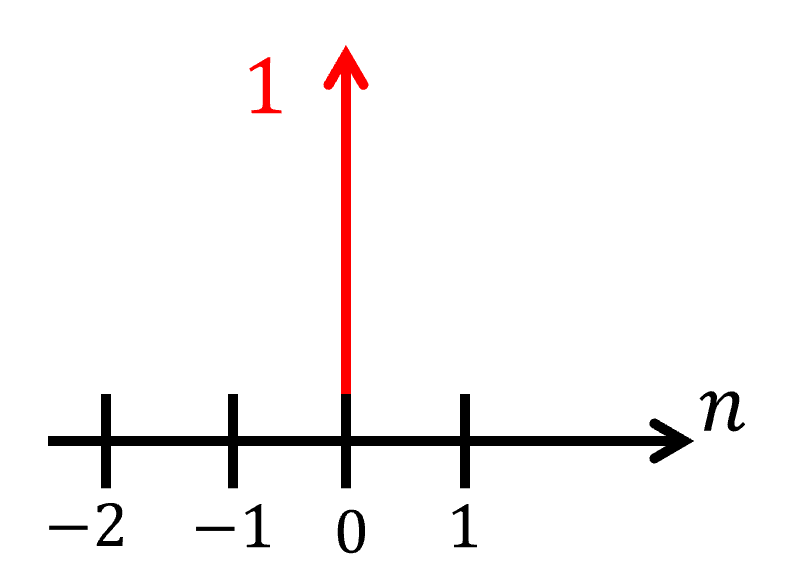
\includegraphics[scale=0.7]{Figuras/pulso_unitario.png}
\end{figure}
\begin{align*}
    \delta[n] = \left\{ \begin{array}{ll}
             1 & n=0\\
             1 & \text{else}
             \end{array}
   \right. 
\end{align*}

\begin{align*}
    x[n]=\sum_{k=0}^{N-1} x_k \delta[n-k]=x_0\delta[n]+x_1\delta[n-1]+x_2\delta[n-2]+...+x_{N-1}\delta[n-(N-1)]
\end{align*}

\begin{align*}
    \{x_n\}_0^{N-1}=\{x_0,x_1,x_2,...,x_{N-1}\} \Longrightarrow \text{Vector de N puntos}
\end{align*}
\begin{figure}[H]
\centering
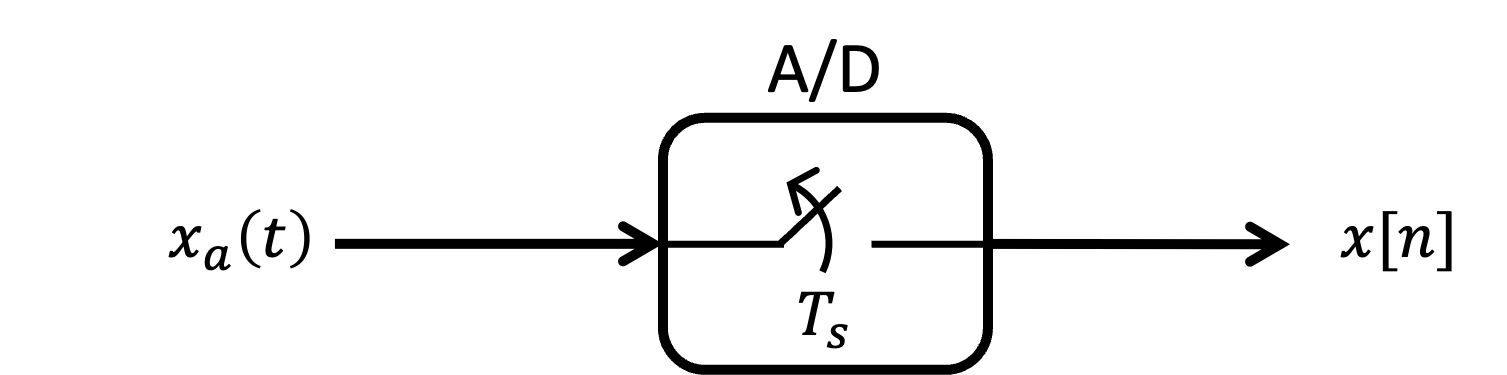
\includegraphics[scale=0.7]{Figuras/AD.png}
\end{figure}


\section{Análisis en frecuencia}
\begin{figure}[H]
\centering
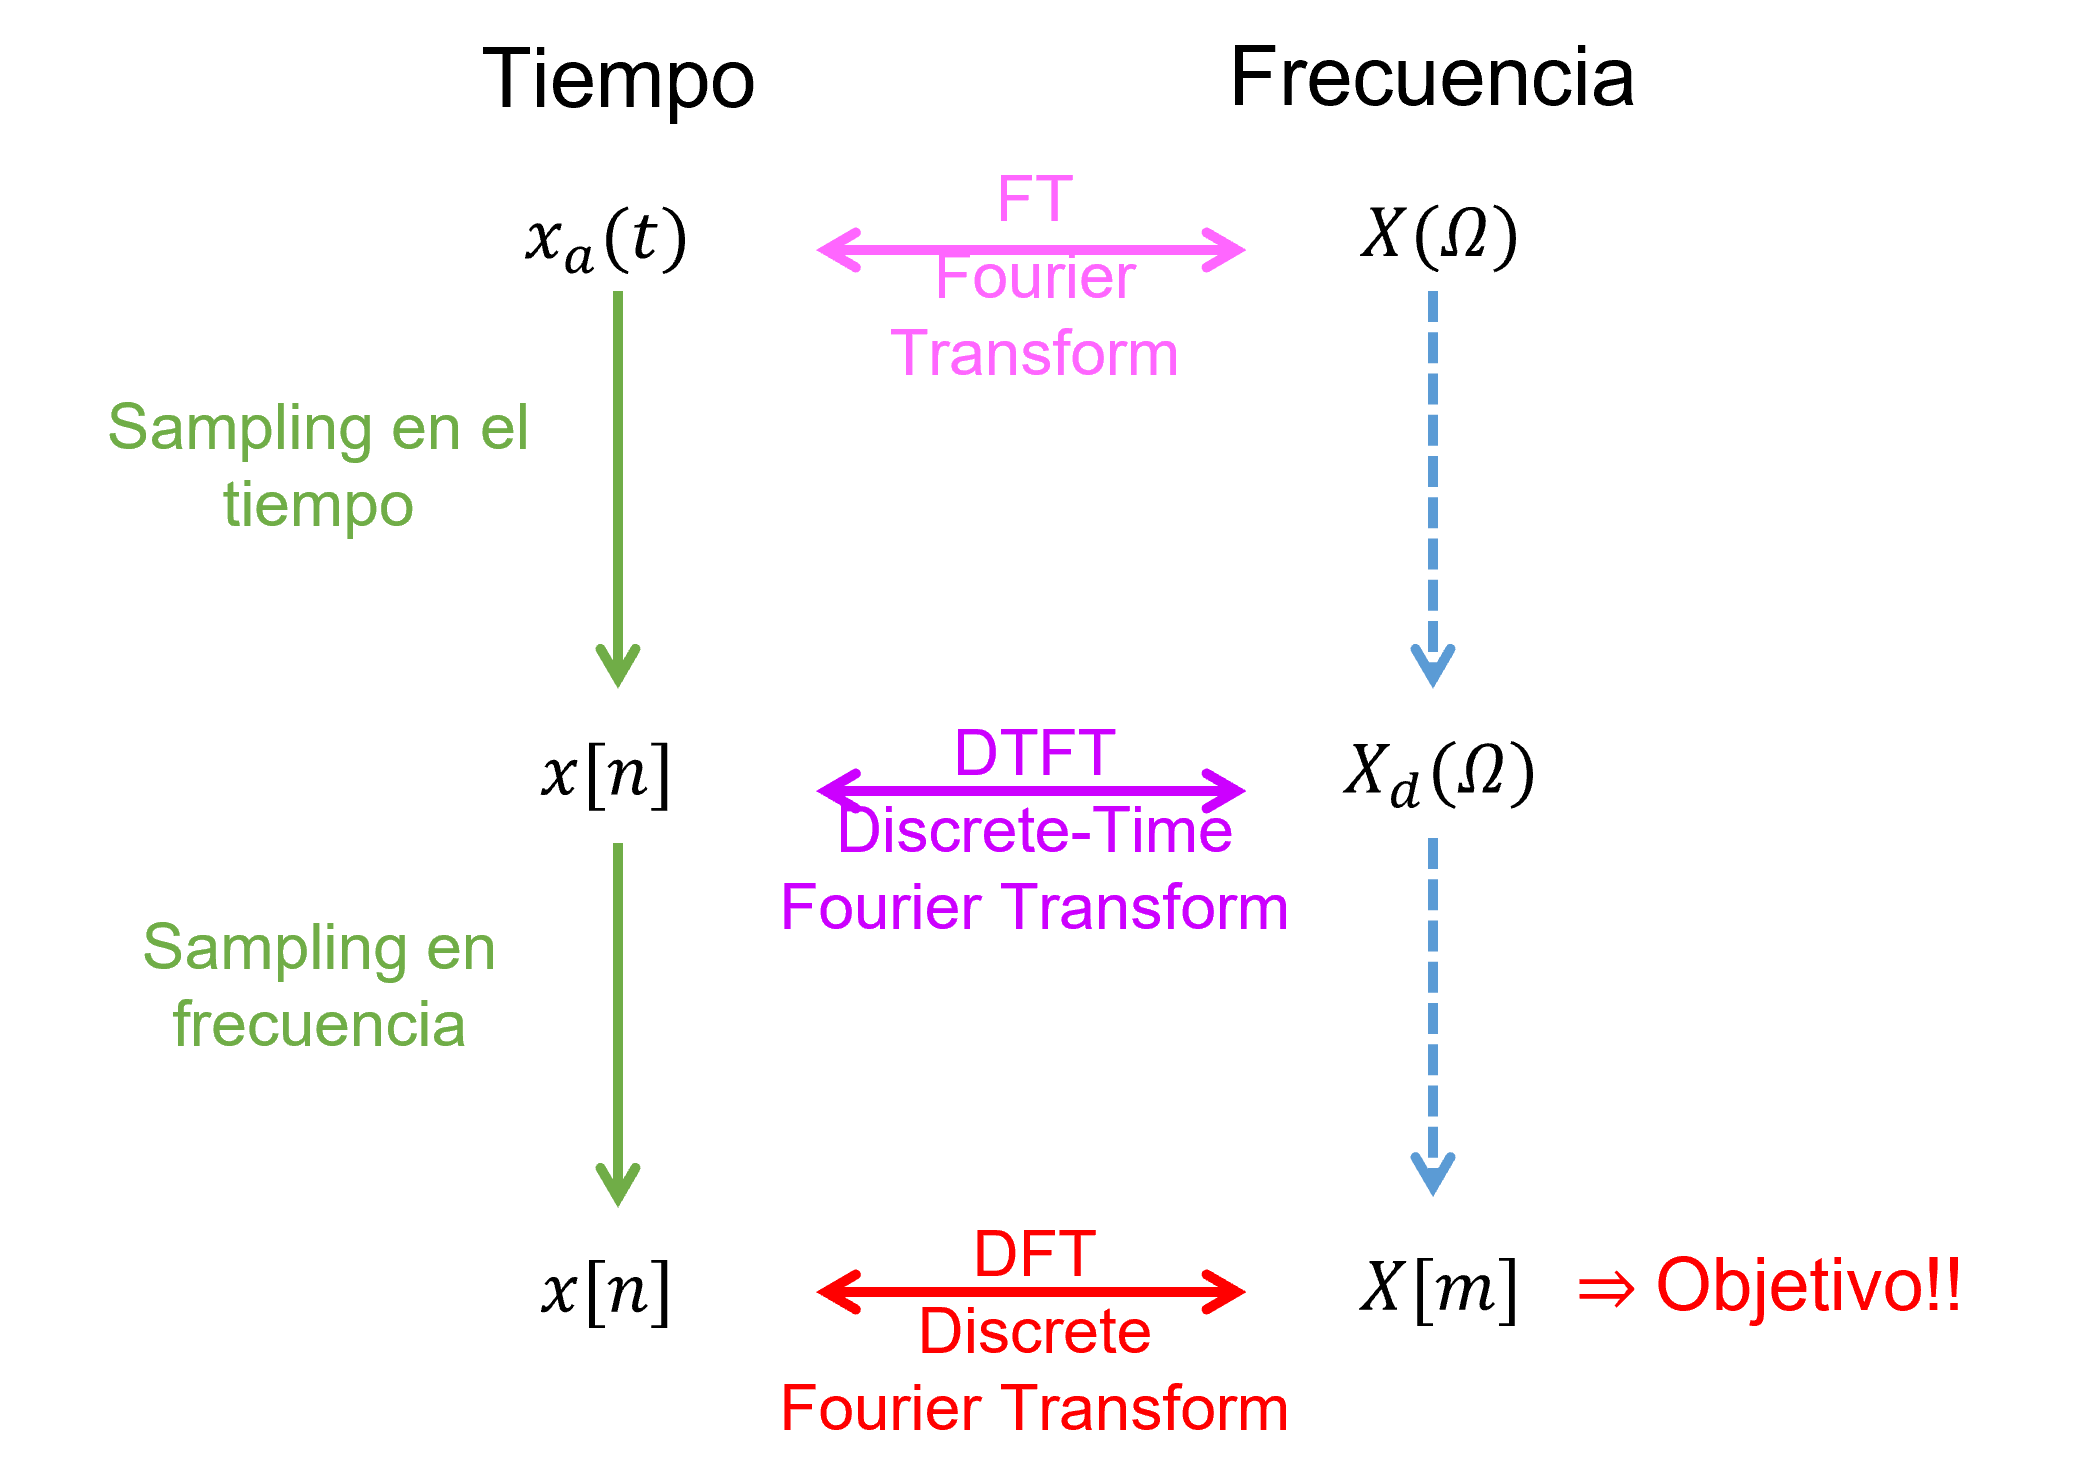
\includegraphics[scale=0.7]{Figuras/analisis_frec.png}
\end{figure}
\par \underline{Fourier Transform (FT)}
\begin{align*}
    X(\Omega) &= \int_{-\infty}^{+\infty}x_a(t)e^{-j\Omega t}dt \quad \text{(FT)}\\
    x_a(t) &= \frac{1}{2\pi}\int_{-\infty}^{+\infty}X(\omega)e^{+j\Omega t}d\Omega \quad \text{(inverse FT)}
\end{align*}

\underline{Nota}: $x_a(t)\in \mathbb{R}$, $X(\Omega)\in \mathbb{C}$, tiene magnitud y fase.\\

\par \underline{Discrete-time Fourier Transform (DTFT)}
\begin{align*}
    X_d(\omega) &= \sum_{n=-\infty}^{\infty}x[n]e^{-j\omega n} \quad \text{(DTFT)}\\
    x[n] &= \frac{1}{2\pi}\int_{-\infty}^{\infty}X_d(\omega)e^{+j\omega n}d\omega \quad \text{(inverse DTFT)}
\end{align*}
$\omega$: variable contínua (frec. DTFT).

\par \underline{Discrete Fourier Transform (DFT)}
\begin{align*}
    \text{(DFT):} \quad X_m &= \sum_{n=0}^{N-1} x_ne^{-j\frac{2\pi}{N}nm}, \quad m\in [0,N-1]\\
    \text{(Inverse DFT):} \quad x_n &= \frac{1}{N}\sum_{m=0}^{N-1}X_me^{+j\frac{2\pi}{N}nm}, \quad n\in[0,N-1]
\end{align*}

\underline{Nota}: Fast Fourier Transform (FFT) es un algoritmo computacional para calcular el DFT.\\
\par \underline{Relación entre DFT y DTFT}
\begin{align*}
    X[m]=X_d\bigg|_{\omega=\frac{2\pi}{N}m}
\end{align*}
\par \underline{Relación entre DTFT y FT}
\begin{align*}
    X_d(\omega)=\frac{1}{T}\sum_{l=-\infty}^{+\infty}X\Bigl(\frac{\omega+wl\pi}{T}\Bigr)
\end{align*}

\section{Criterio de muestreo de Nyquist}
En DSP, queremos muestrear la señal sin pérdida de información (``loss less'').\\
\par Entonces, hay que elegir correctamente el intervalo de muestreo T (sampling time).\\

\par \underline{Teorema de Nyquist}
La frecuencia de muestreo de una señal análoga debe ser al menos el doble de la máxima frecuencia de la señal: $$F_s>2f_{max} $$



\section{Aliasing}

Aliasing es un fenómeno que ocure cuando el terorema de Nyquist no se cumple $\Longrightarrow$ Ocurre cuando una señal análoga no puede ser reconstruida por la señal digitalizada.\\

\underline{Ejemplo}: 
\begin{figure}[H]
\centering
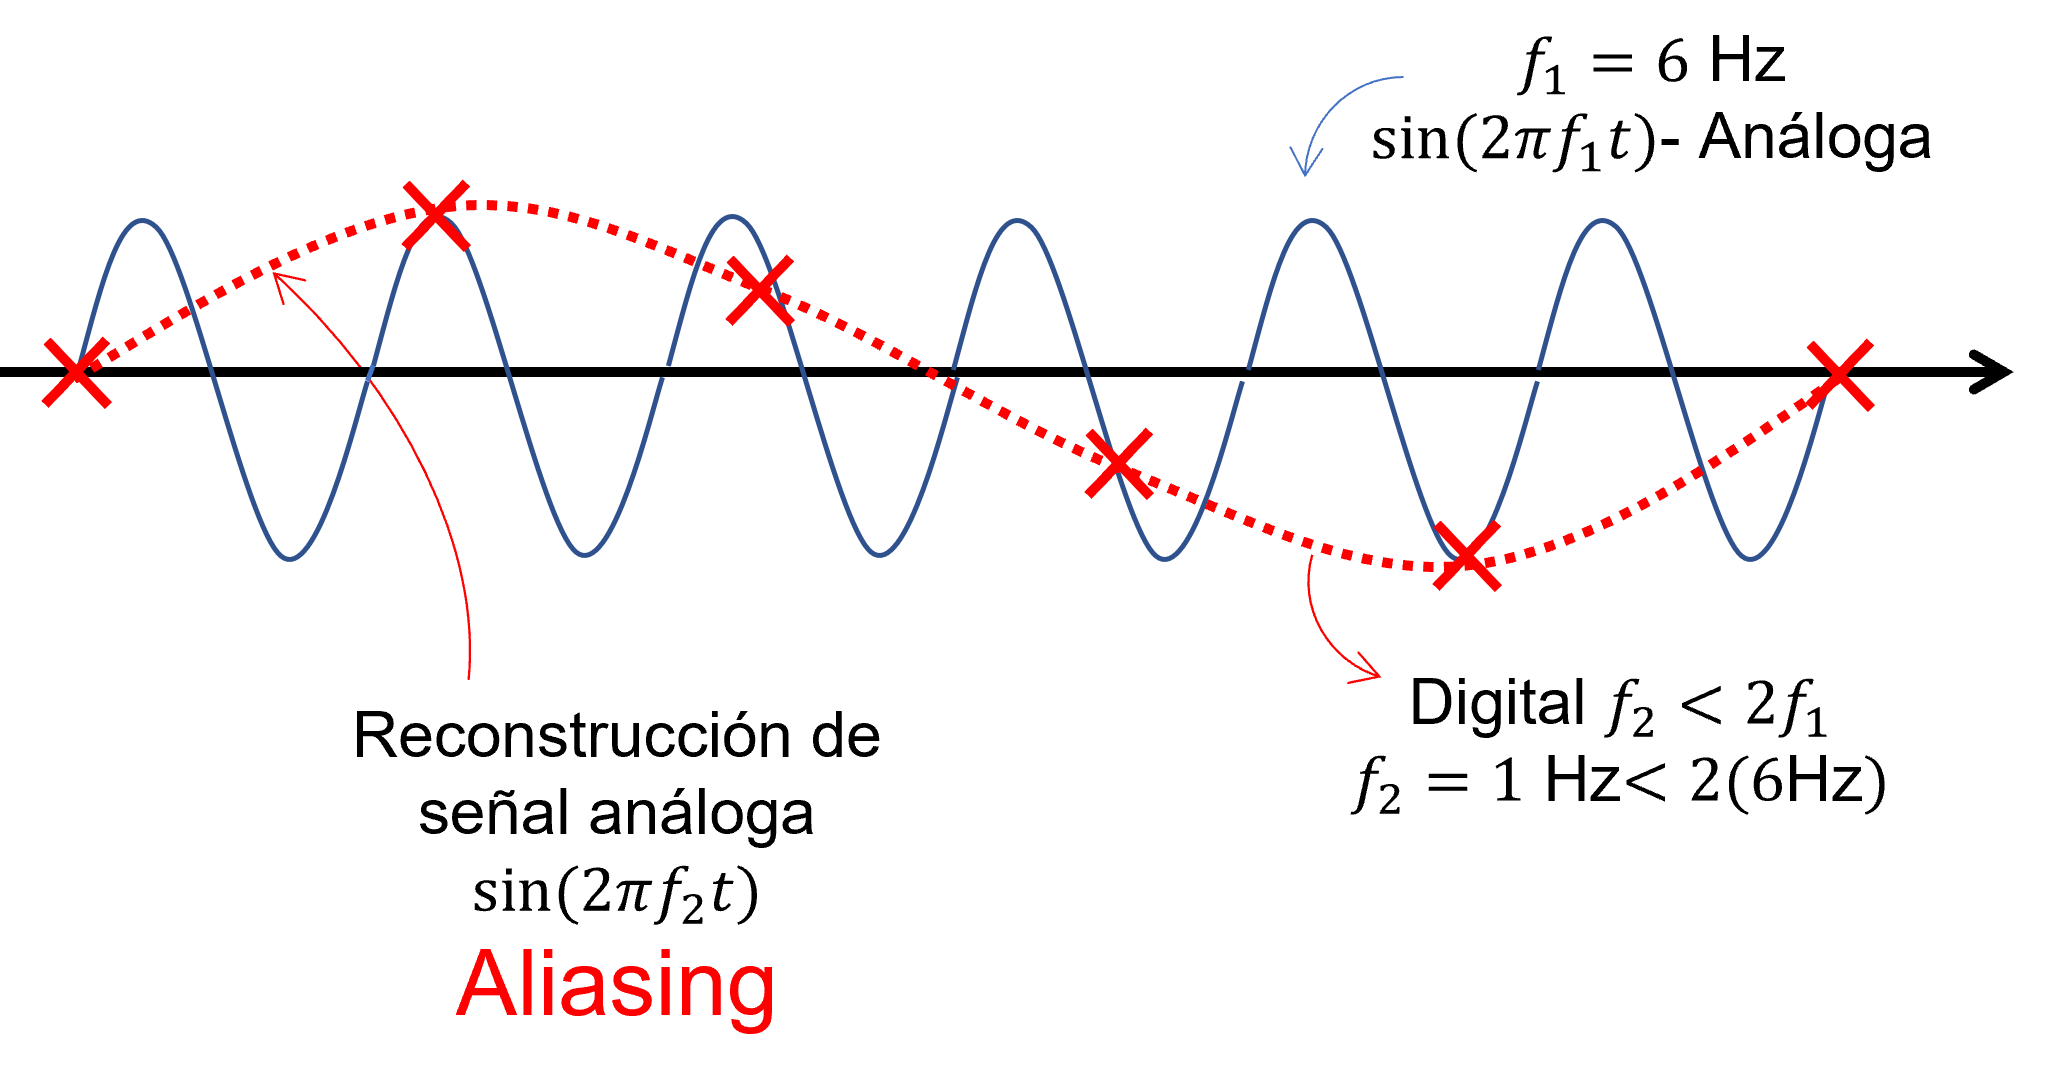
\includegraphics[scale=0.7]{Figuras/aliasing.png}
\end{figure}

\subsection{Aliasing en dominio de frecuencia}
Sin Aliasing:

\begin{figure}[H]
\centering
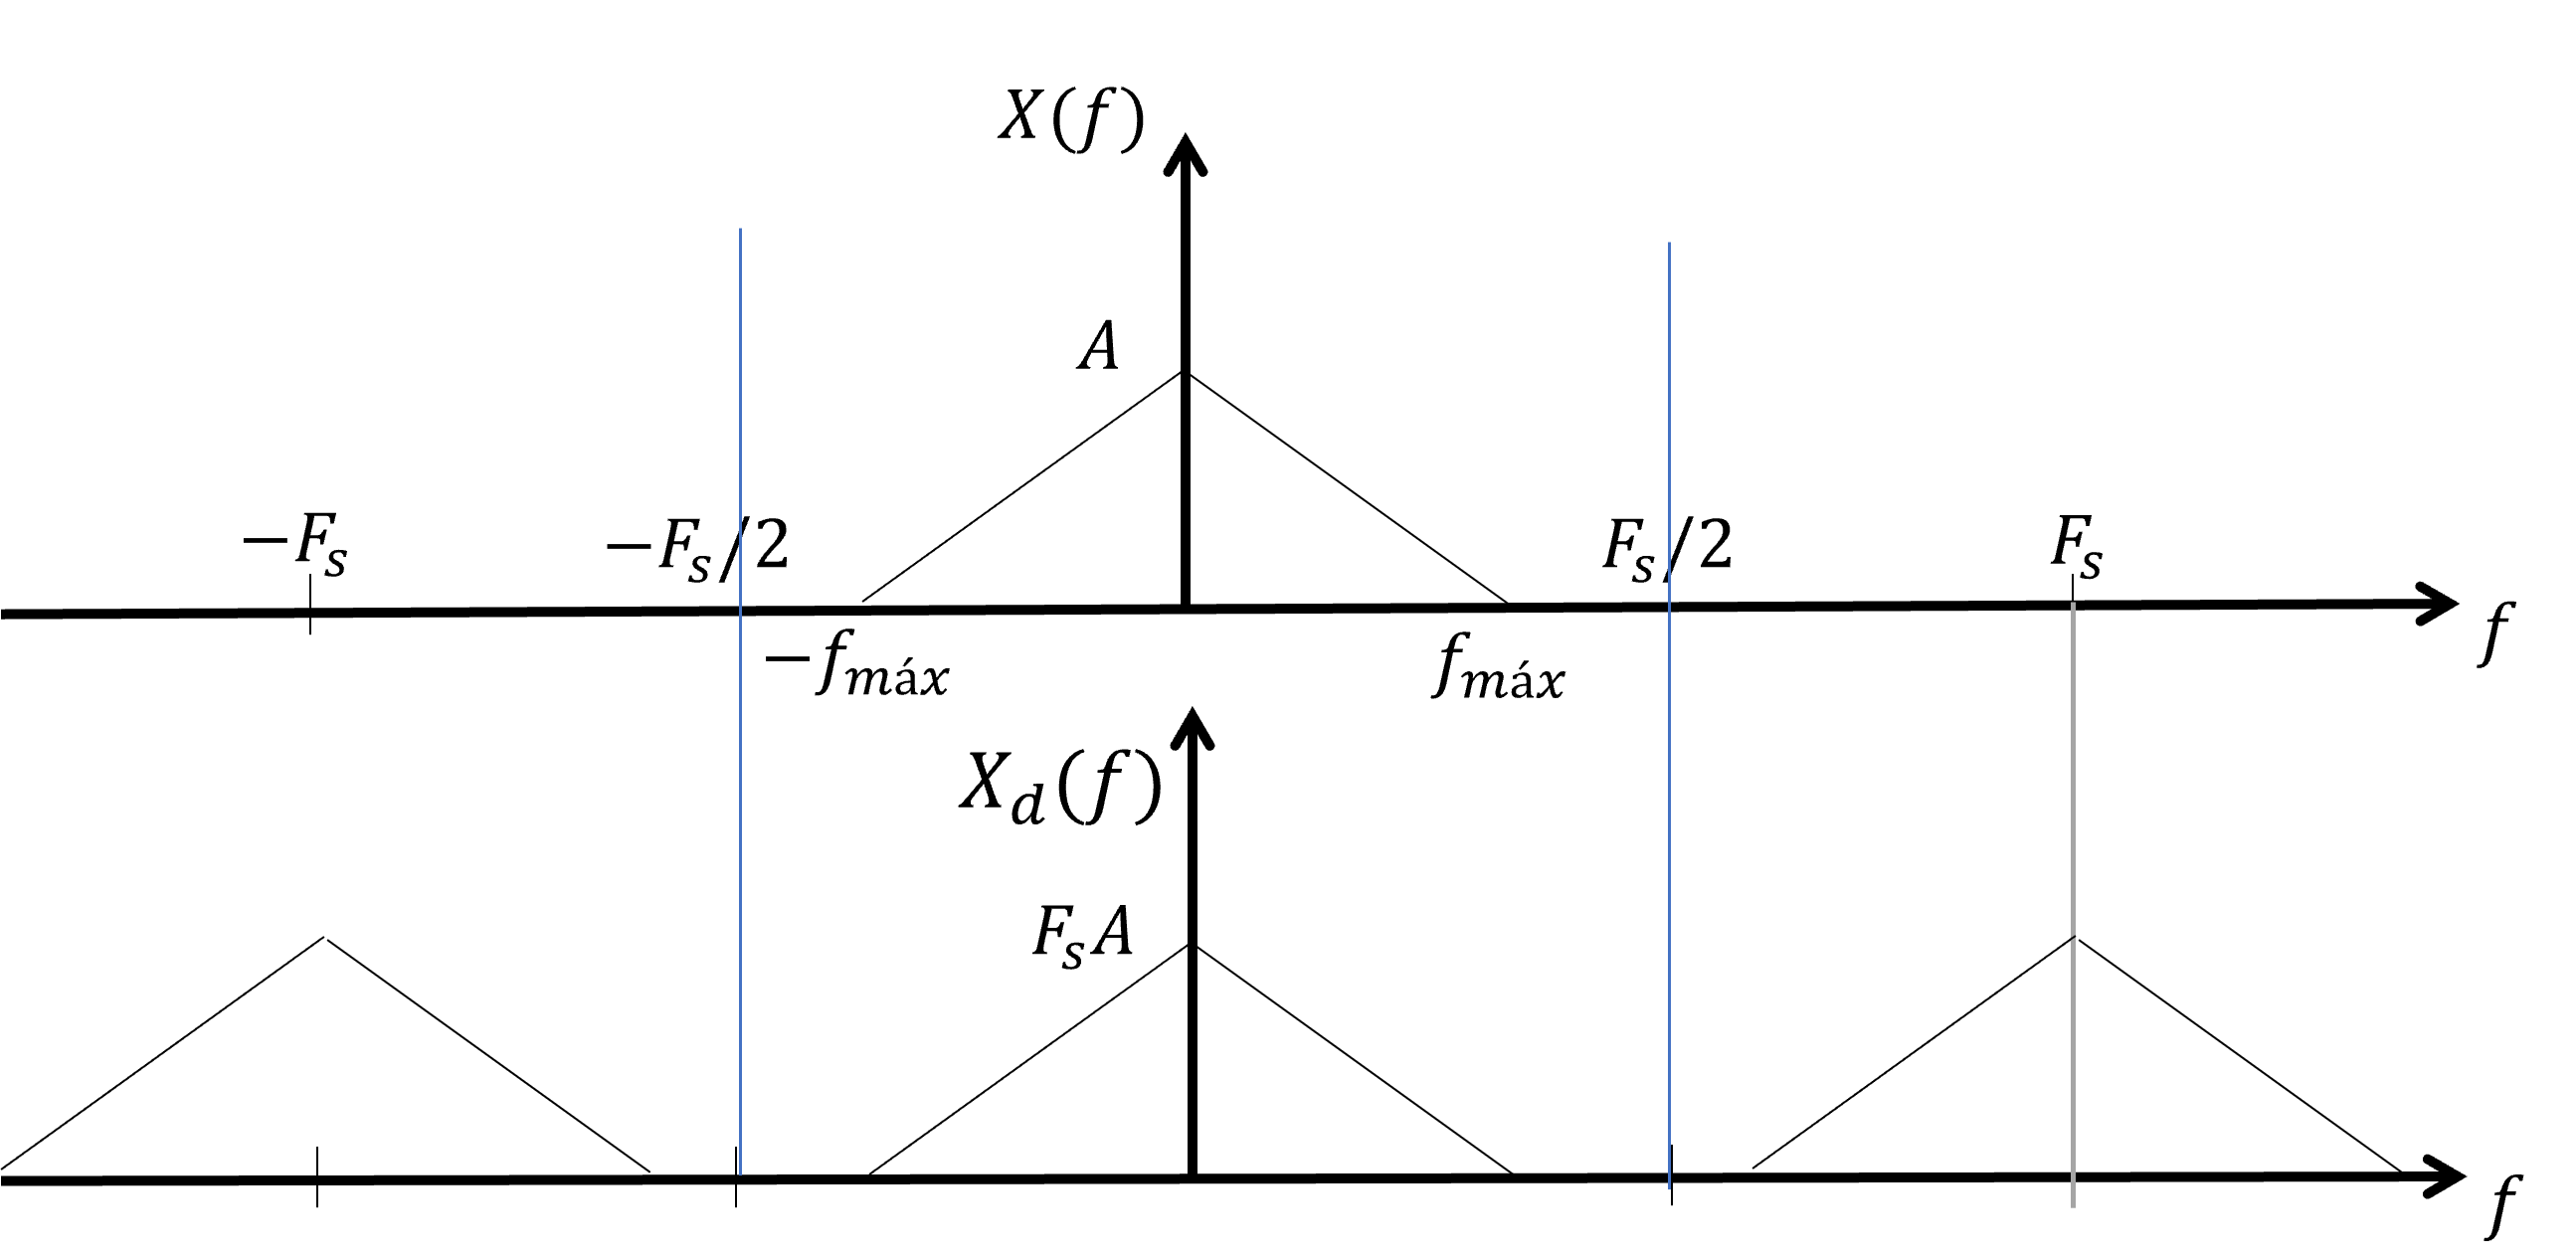
\includegraphics[scale=0.7]{Figuras/sin_aliasing.png}
\end{figure}

\begin{align*}
    Fs &> 2f_{max}\\
    f_{max} &< \frac{Fs}{2}=F_N \quad \text{frecuencia de Nyquist}
\end{align*}

\par Con Aliasing:

\begin{figure}[H]
\centering
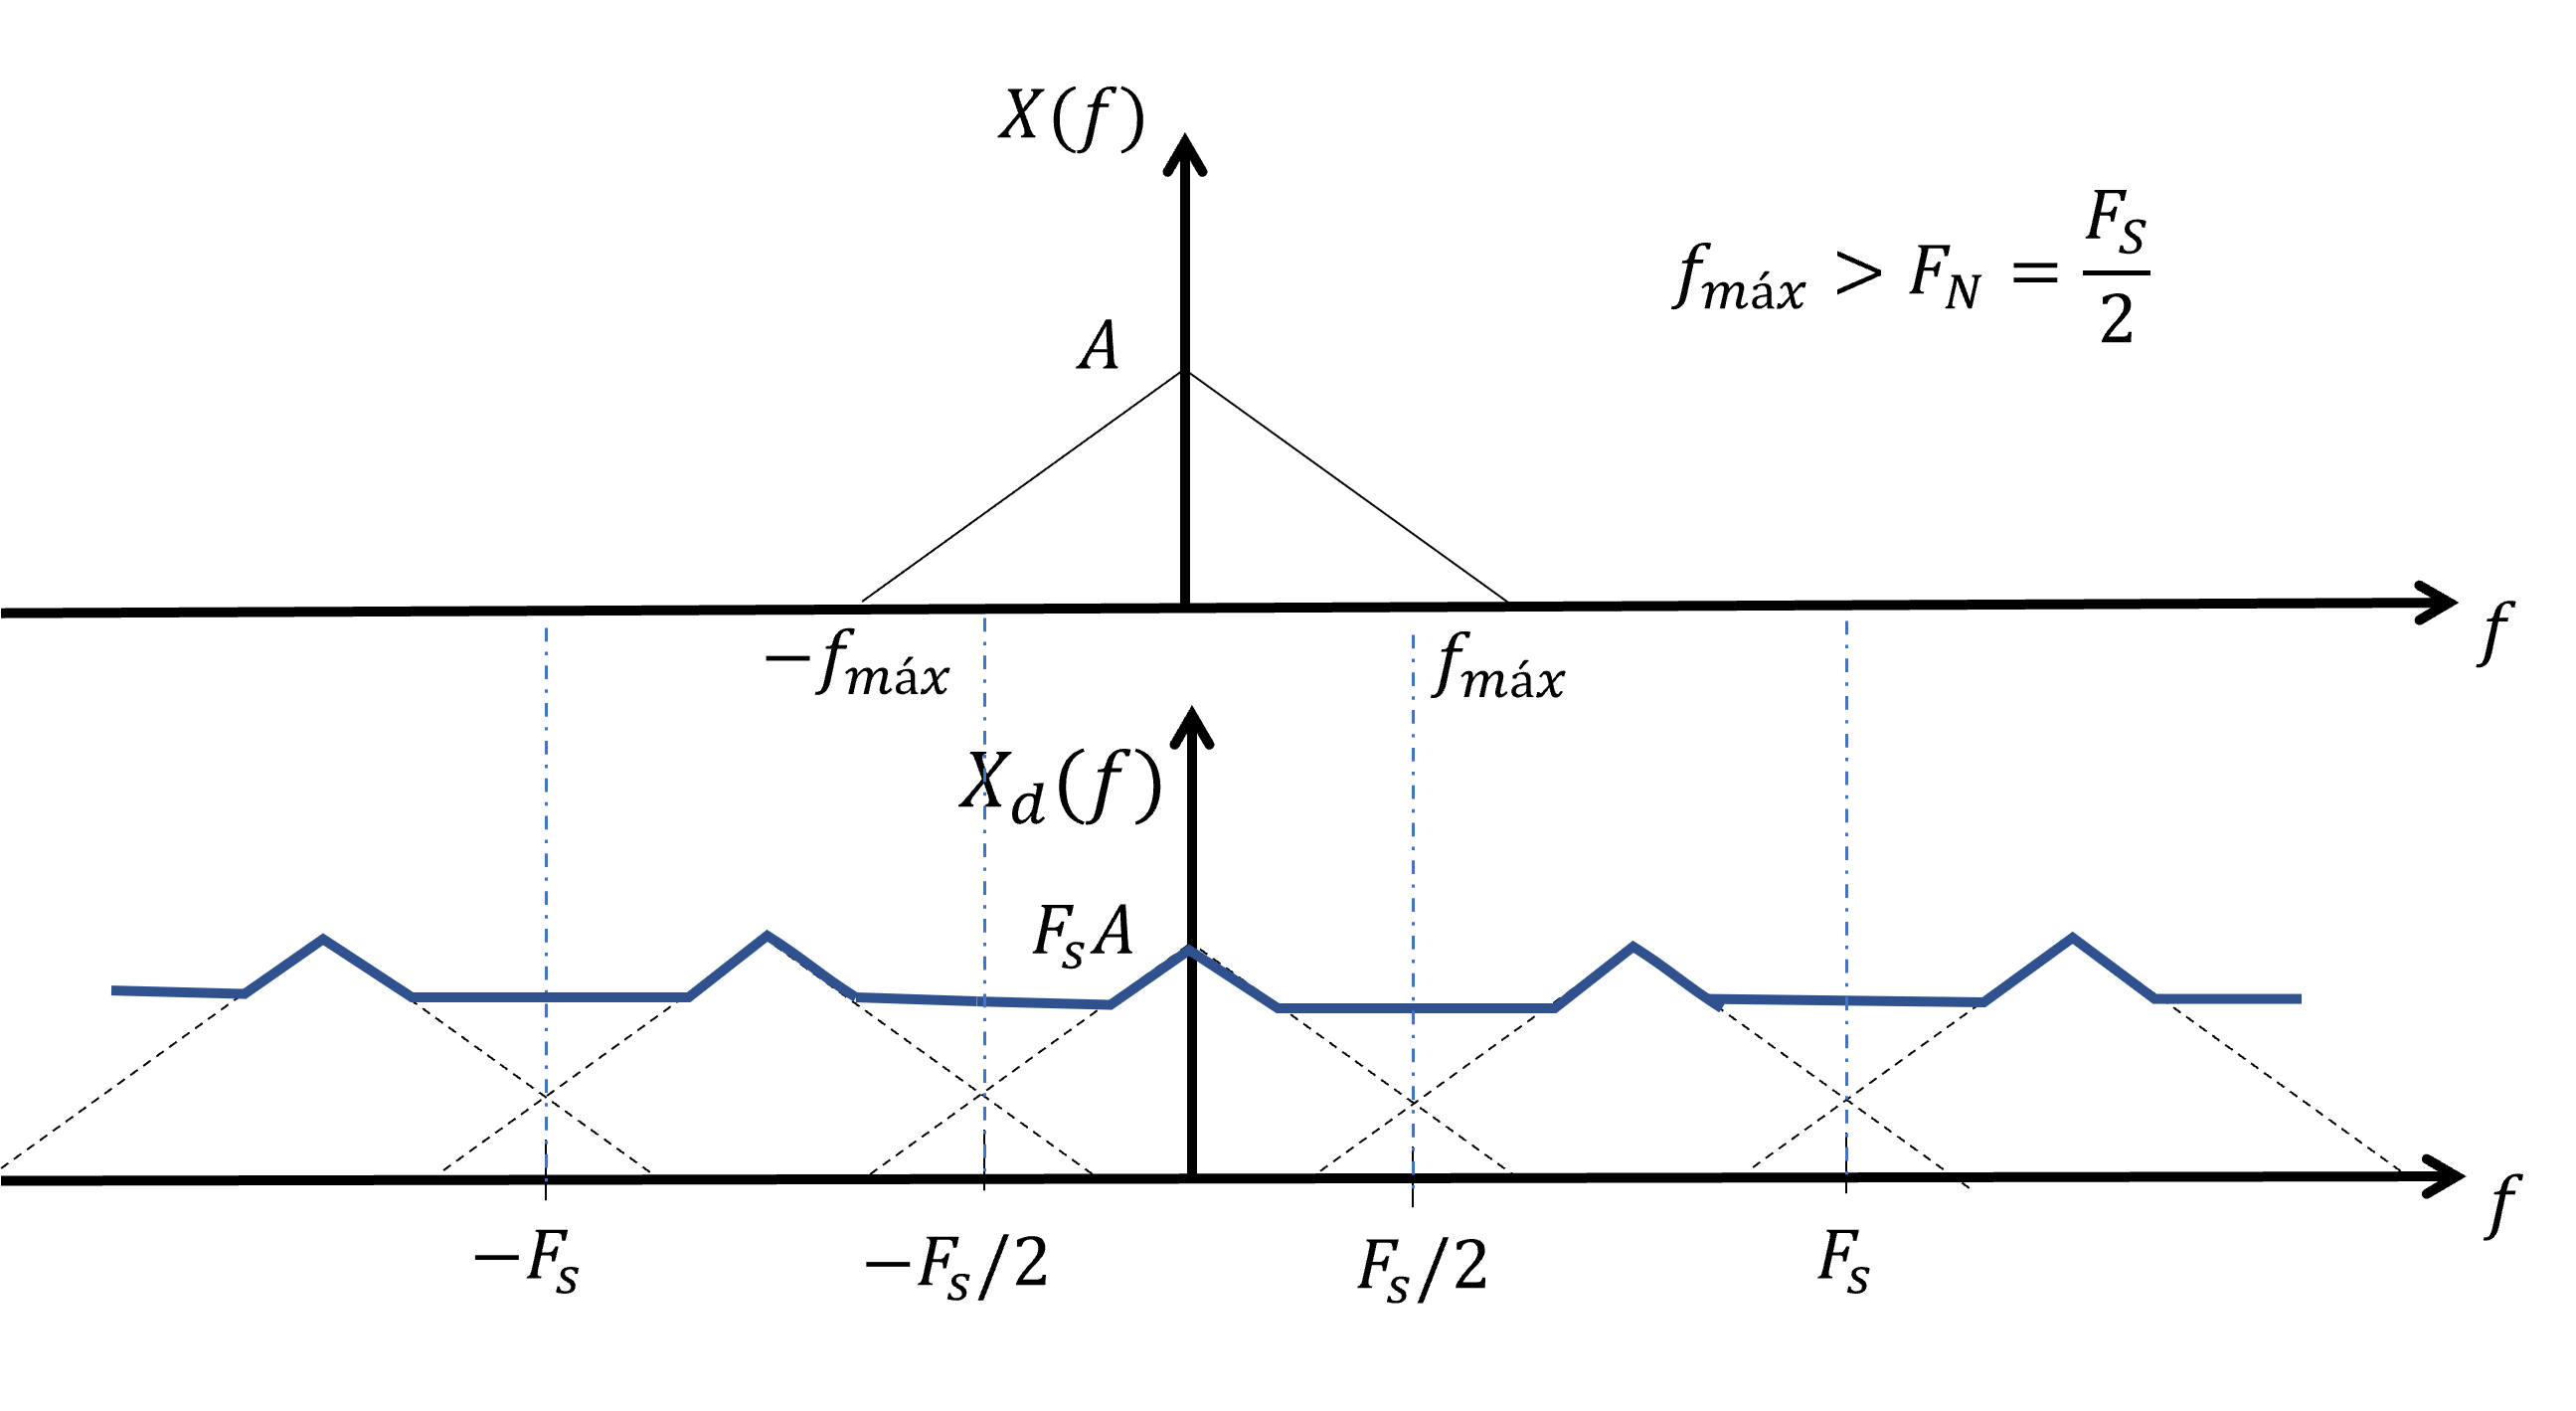
\includegraphics[scale=0.7]{Figuras/con_aliasing.png}
\end{figure}

\begin{figure}[H]
\centering
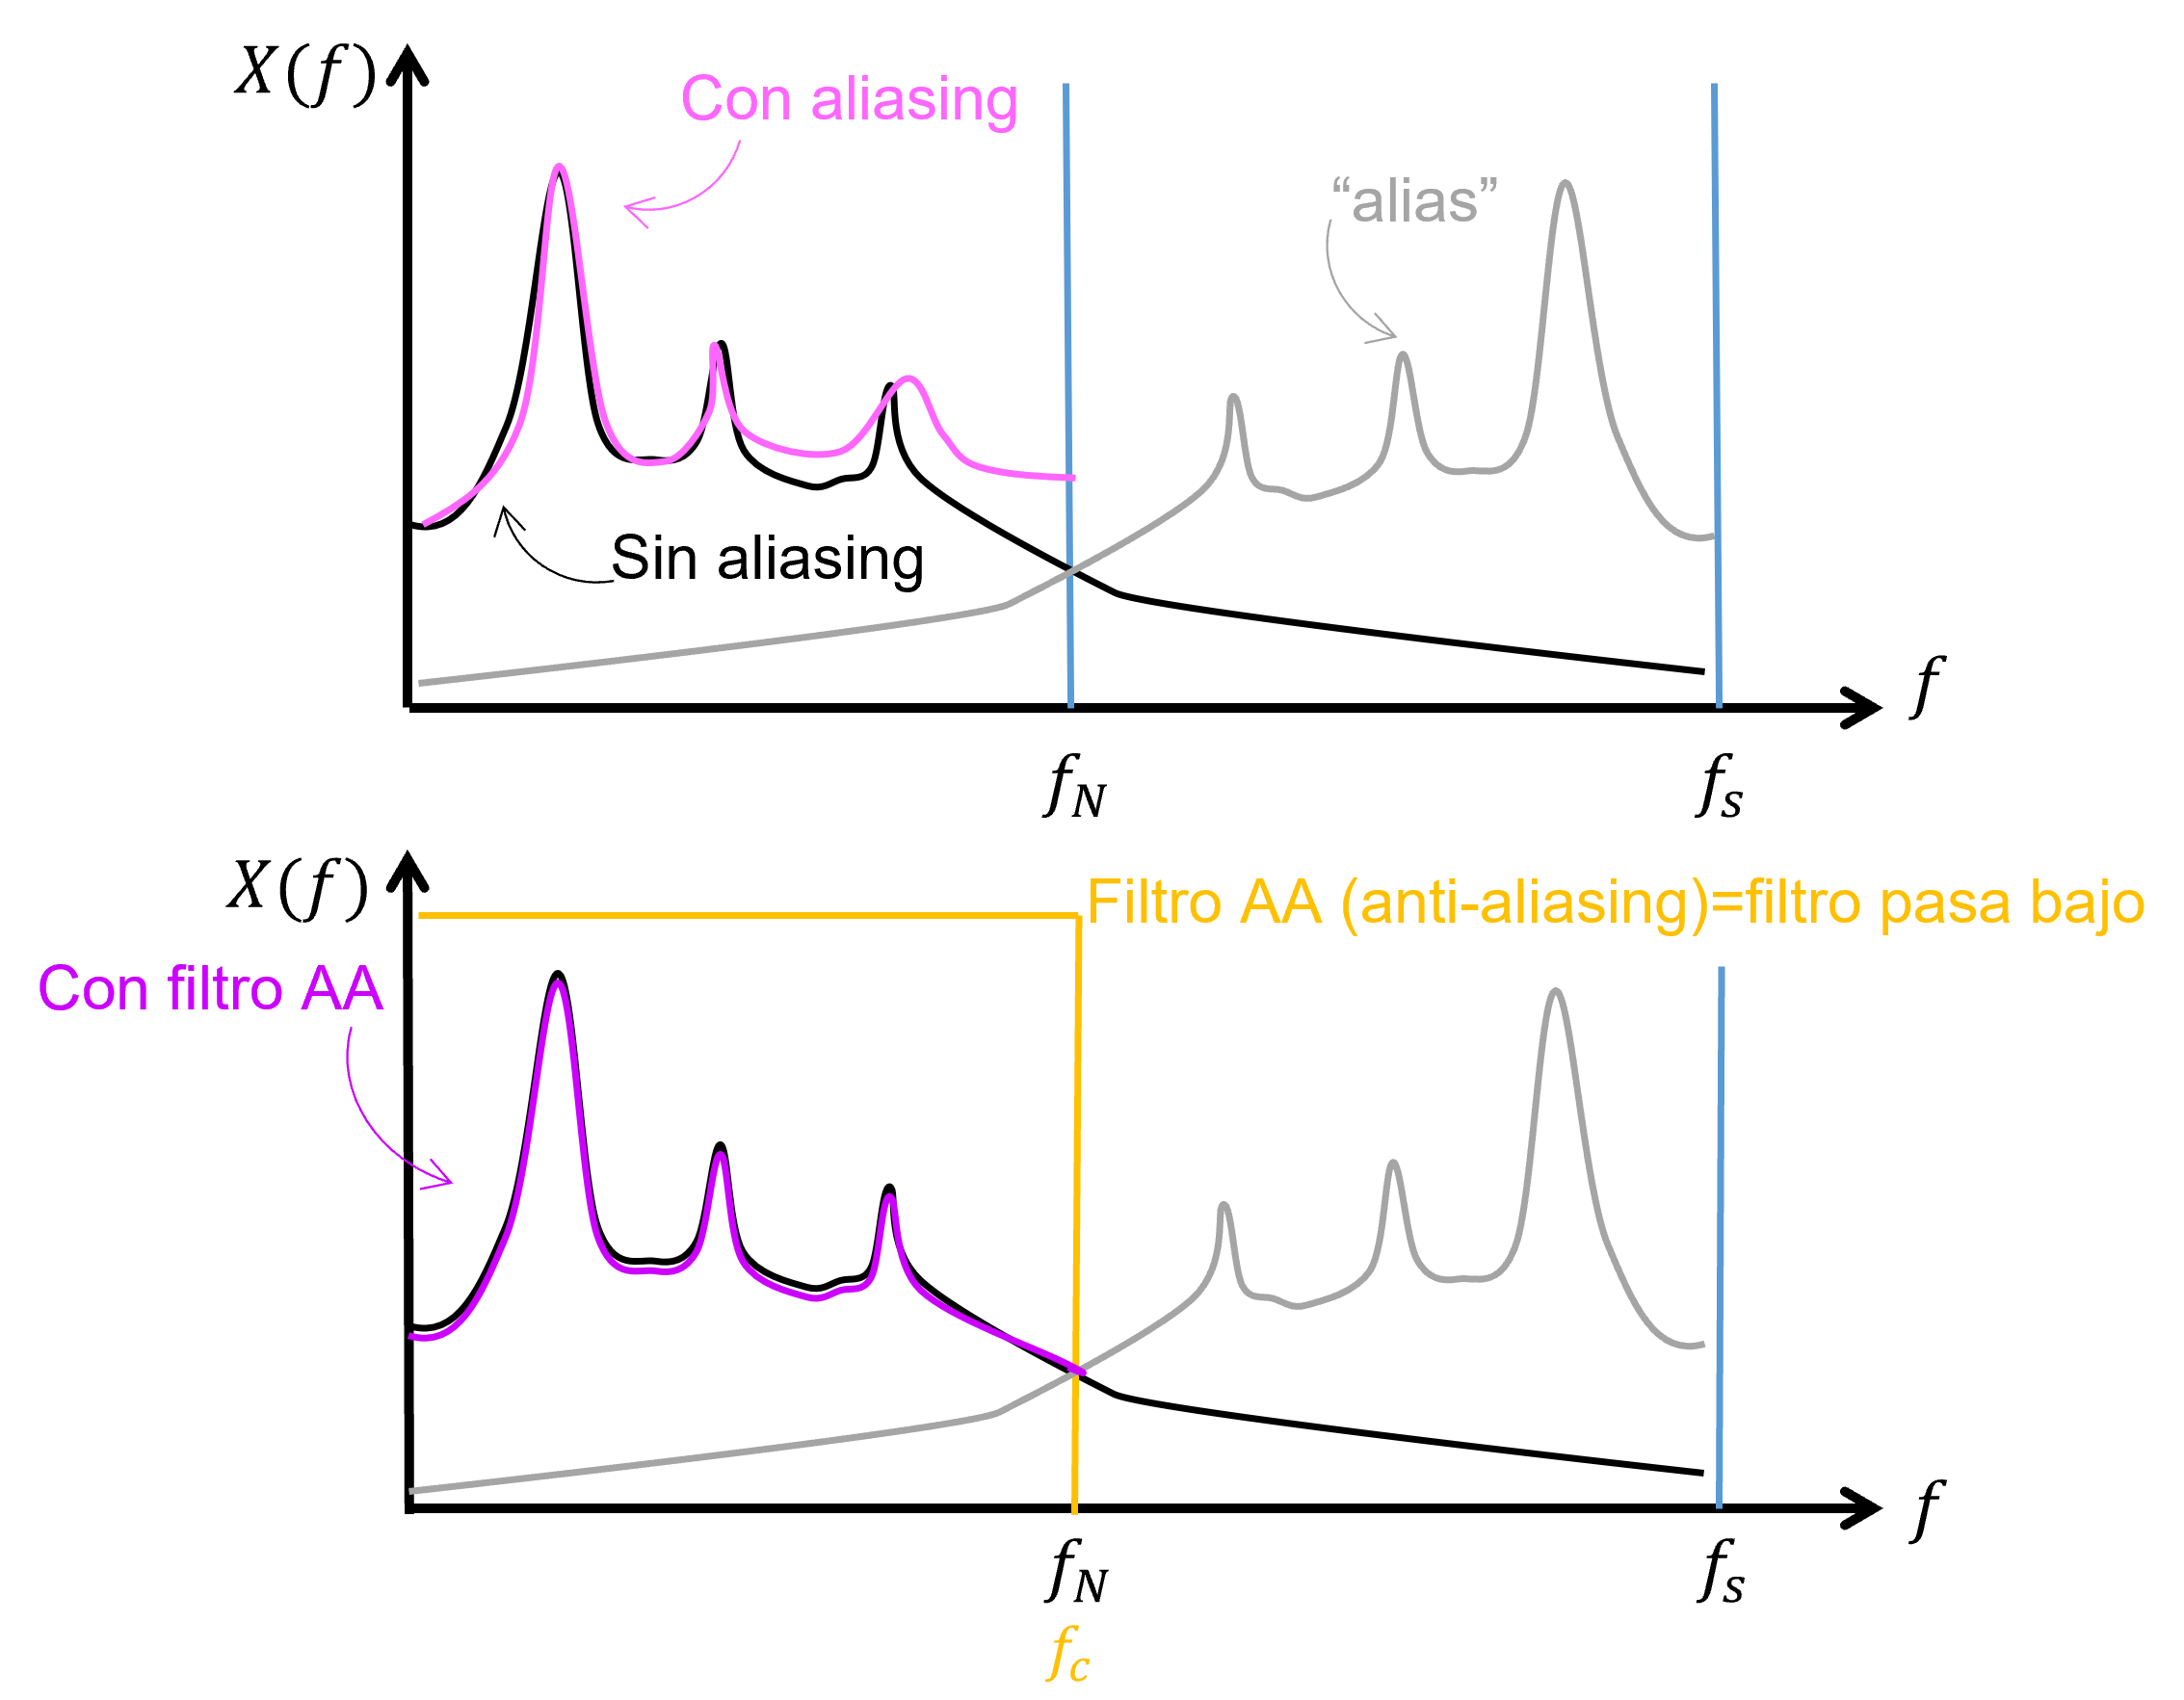
\includegraphics[scale=0.7]{Figuras/filtroAA.png}
\end{figure}

\begin{itemize}
    \item Filtro anti-aliasing es utilizado para eliminar el ``aliasing'' de la respuesta en frecuencia.
    \item Filtro AA tiene que ser aplicado antes del muestreo en el tiempo.
\end{itemize}

\begin{figure}[H]
\centering
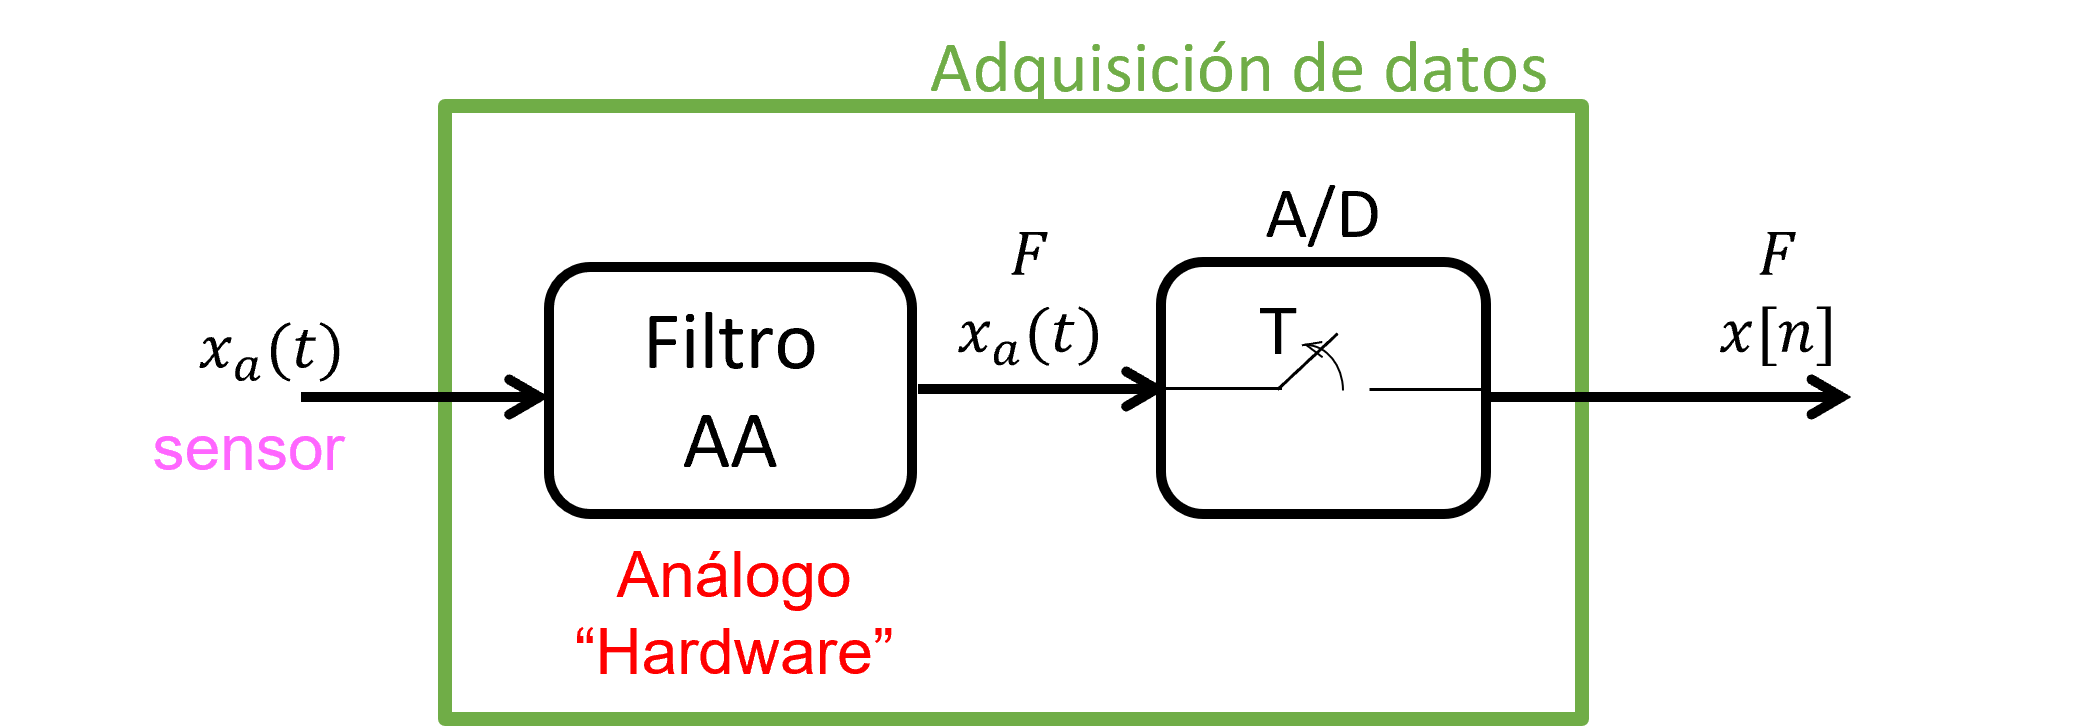
\includegraphics[scale=0.7]{Figuras/filtroAA2.png}
\end{figure}

\subsection{Spectral Leakage}
FT/DTFT/DFT asume que la señal es del tipo periódica.
$$ x(t) = x(t+T_1) $$
¿Qué pasa con señales no periódicas?
\begin{figure}[H]
\centering
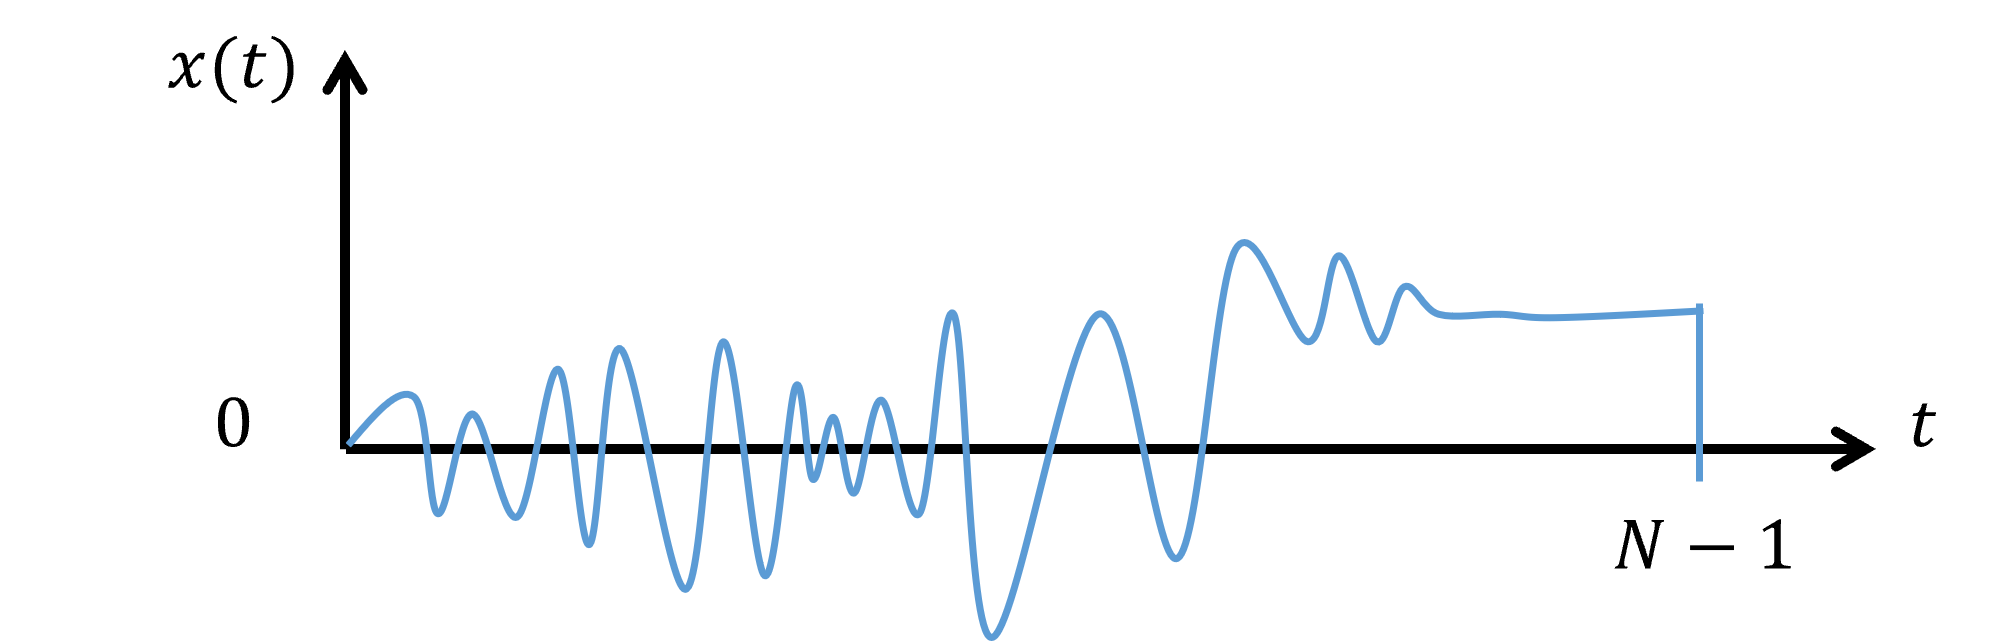
\includegraphics[scale=0.7]{Figuras/FT.png}
\end{figure}
DFT (N-pts): $X[m]=\sum_{n=0}^{N-1}x[n]e^{-j2\pi/N nm}$, $n$: 
indice tiempo, $m$: índice frecuencia
\begin{figure}[H]
\centering
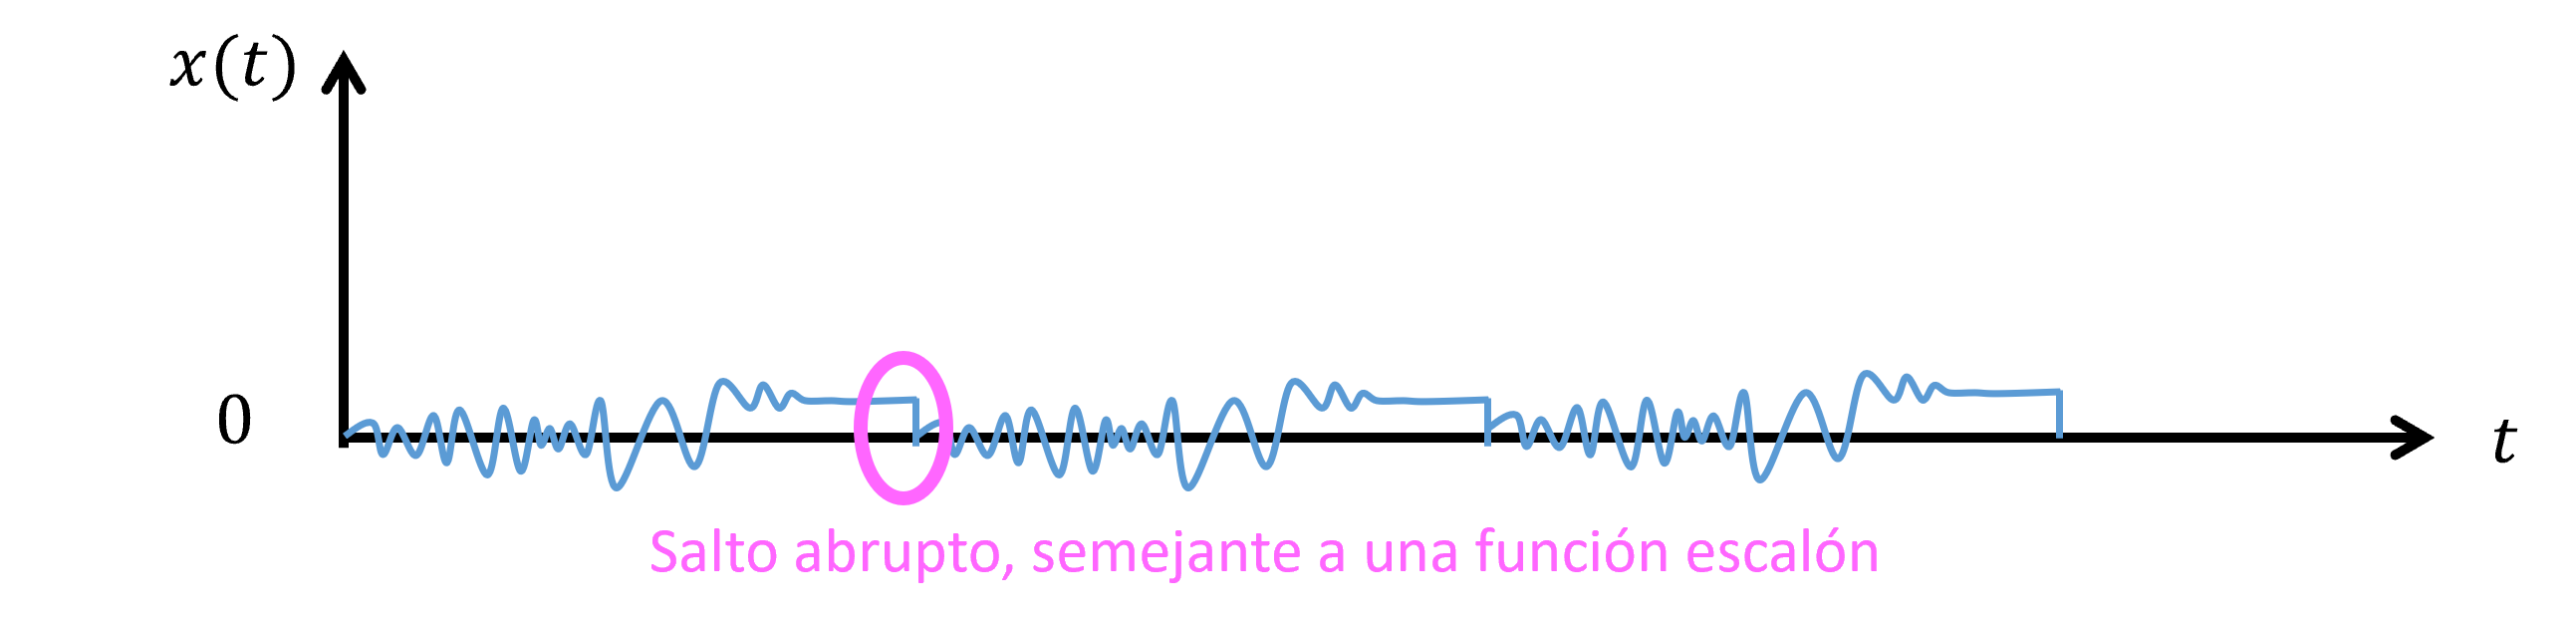
\includegraphics[scale=0.7]{Figuras/DFT.png}
\end{figure}

\par Una función escalón se puede escribir como una serie de Fourier (suma de armónicas).\\

\par Al calcular $X[m]$ (DFT de $x[n]$) surge el fenómeno de ``spectral leakage'', donde se agregan armónicas artificiales producto del escalón generado.\\
\par \underline{Ejemplo}:

\begin{figure}[H]
\centering
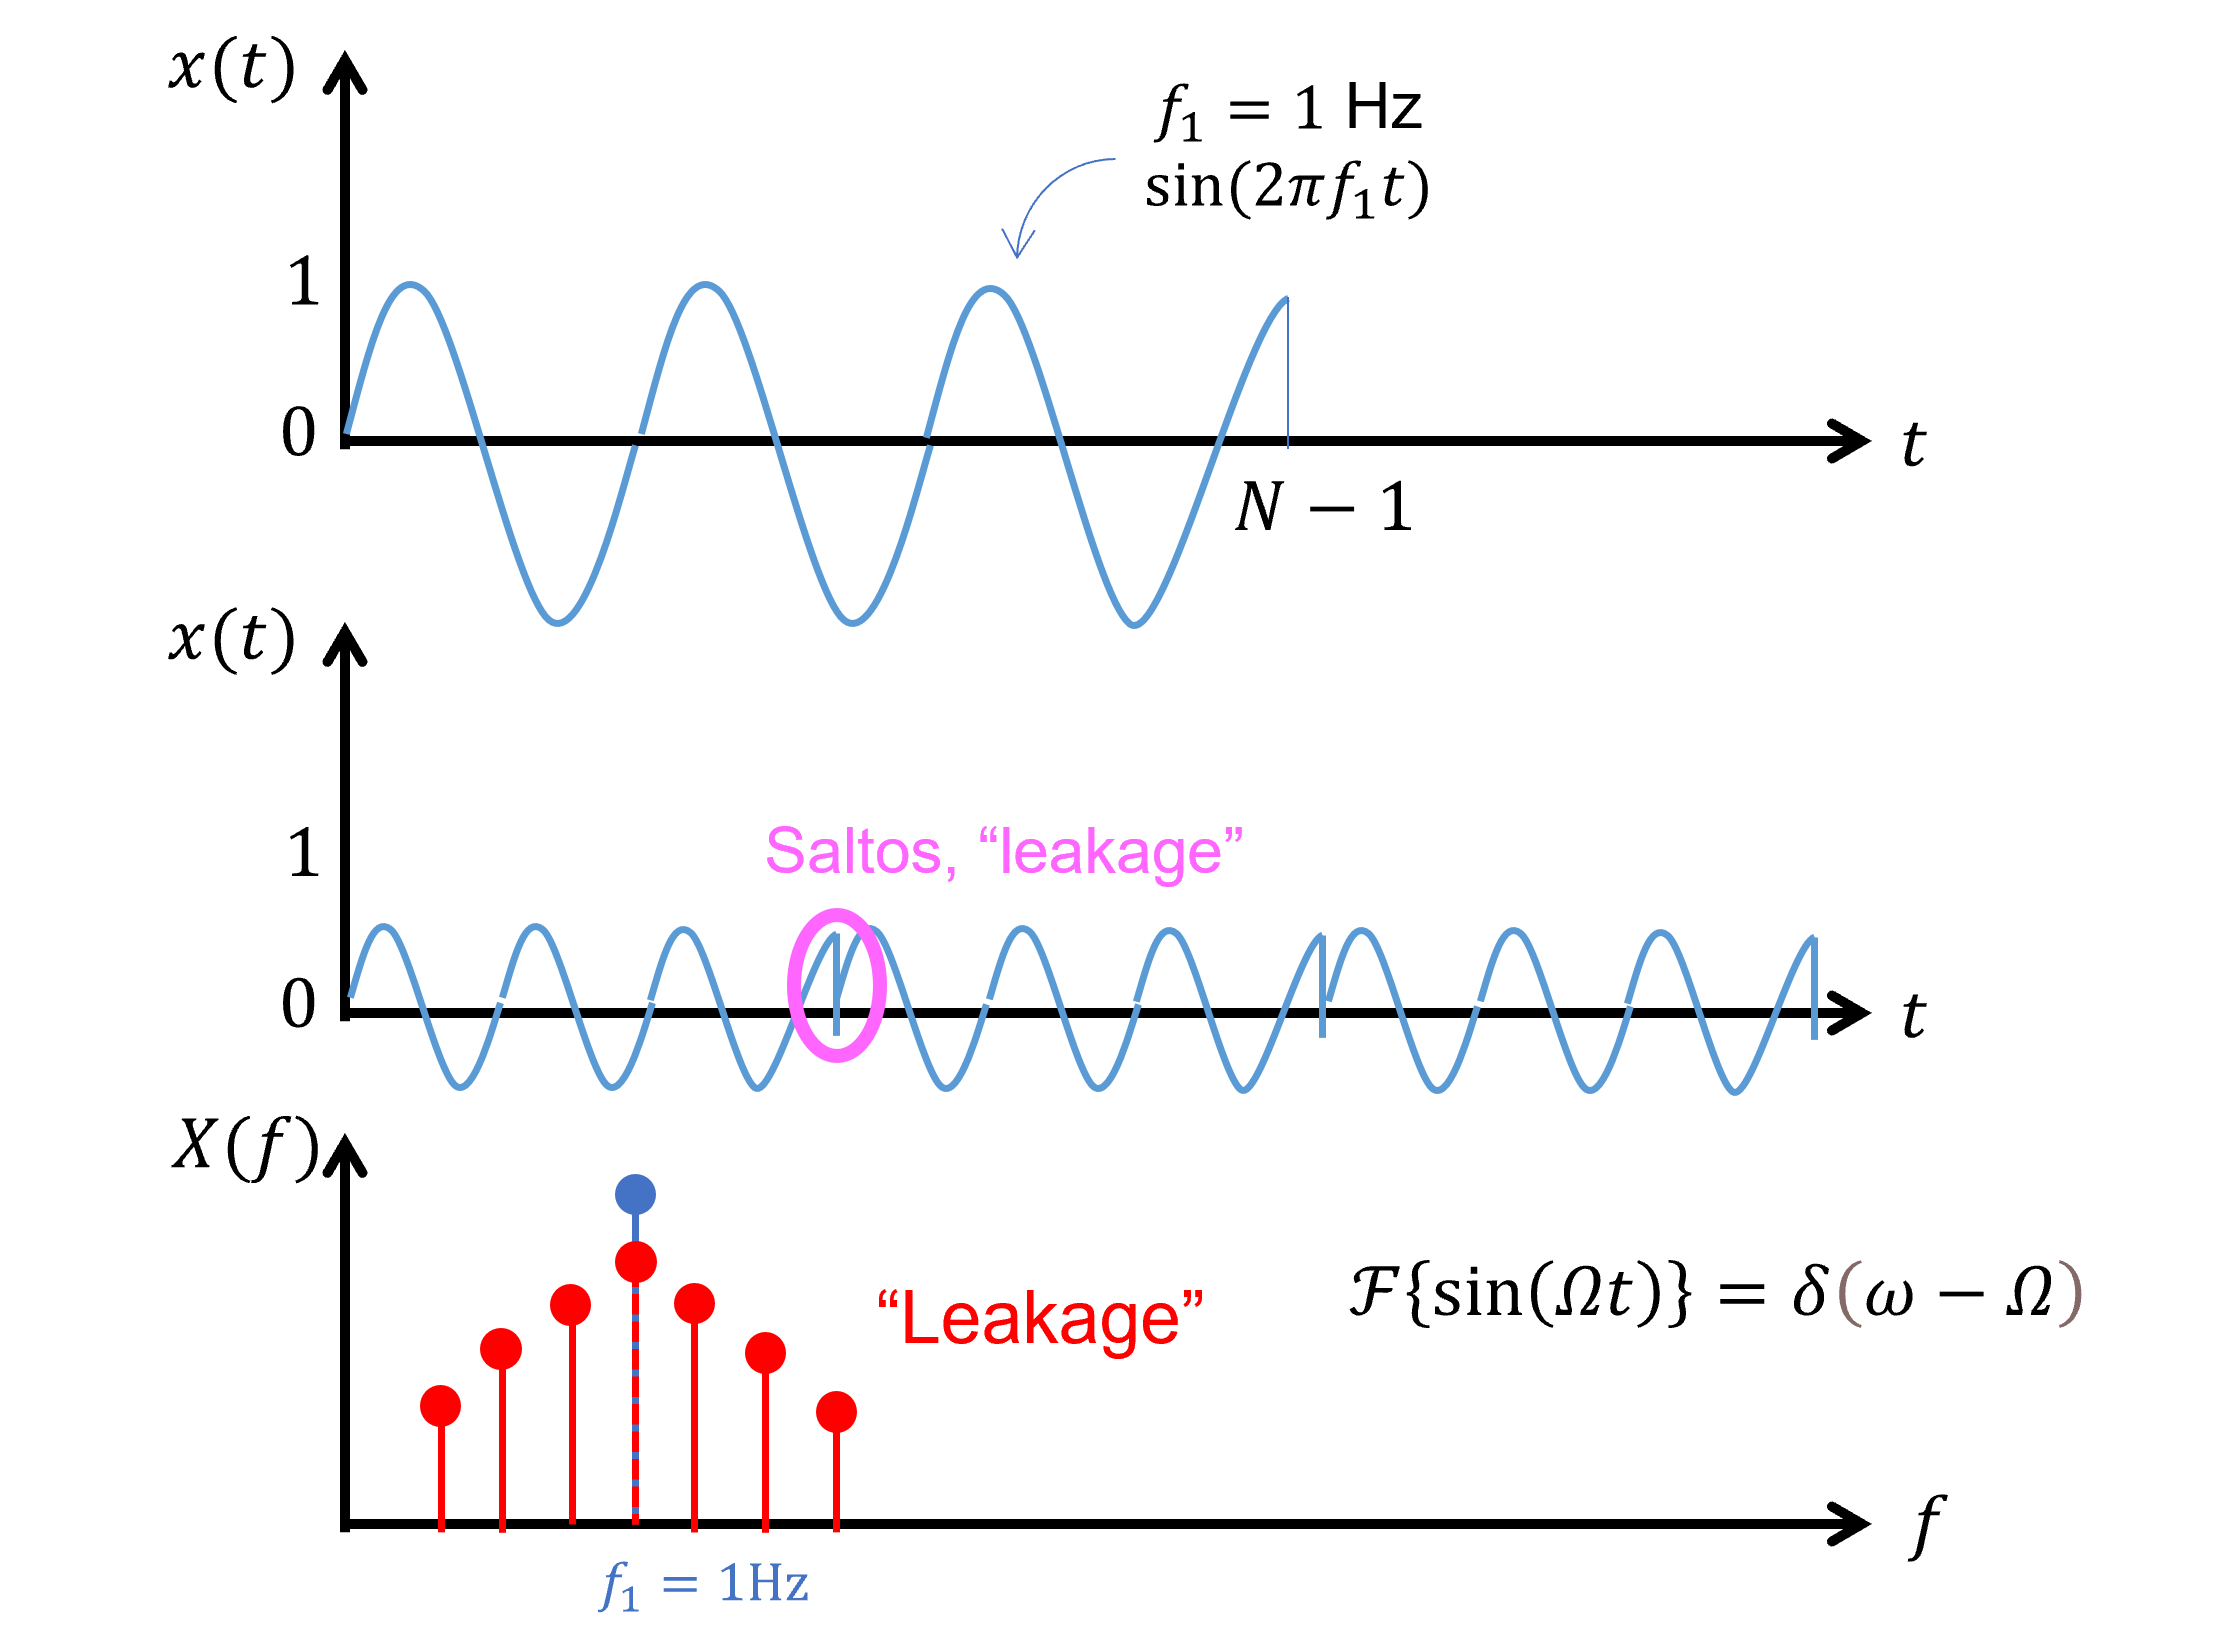
\includegraphics[scale=0.7]{Figuras/ejemplo_leakage.png}
\end{figure}

\par \underline{Solución}: ``Windowing'' $\Longrightarrow$ aplicar ventanas.\\
\par Sobre el cálculo de PSD en registros digitales: 

\begin{figure}[H]
\centering
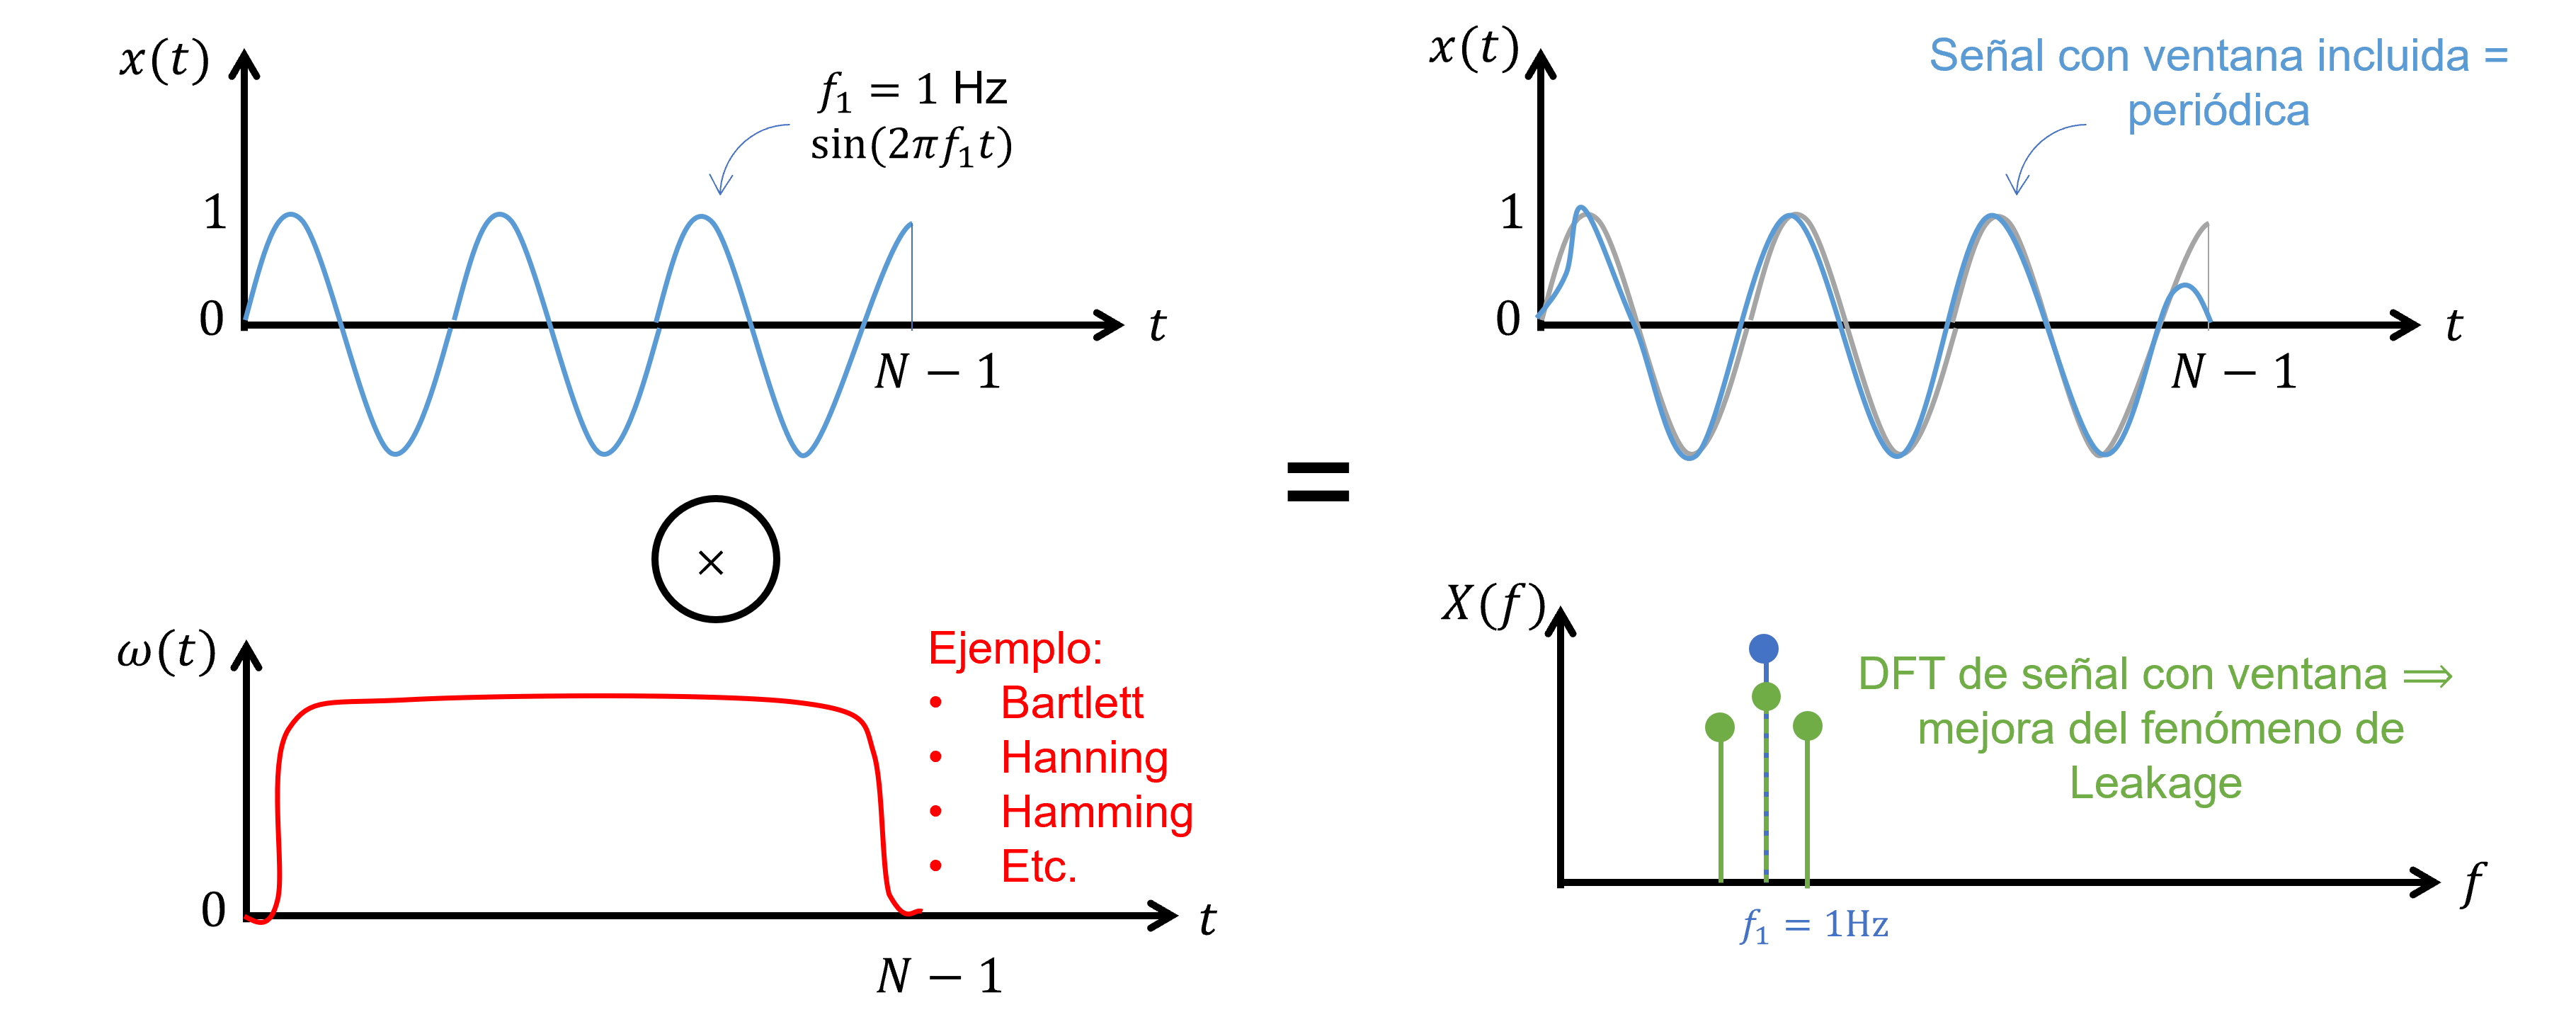
\includegraphics[scale=0.6]{Figuras/solucion_leakage.png}
\end{figure}

\begin{align*}
    u(t)\xrightarrow[]{\text{Auto-PSD}} S_{UU}(\omega)=\mathcal{F}\{R_{UU}(\tau)\}\\
    \Longrightarrow S_{UU}(\omega) = \mathcal{F}\Bigl\{\mathbb{E}\{u(t)u(t+\tau)\}\Bigr\}
\end{align*}

Cómo calcular $S_{UU}(\omega)$ con una señal digital? $\Longrightarrow$ Periodograma.


\section{Motivación}
Sea $x[k]$ un proceso estocástico wss (estacionario sentido amplio), señal digital con un intervalo de muestreo T.
\begin{align*}
    S_X(\omega) &= \mathbb{F}\{R_x(\tau)\} \quad \text{(Caso contínuo)}\\
    &= \mathbb{E}\{X(\omega)X^\ast(\omega)\} \quad \text{(Caso contínuo)}
\end{align*}

Podemos estimar $S_x(\omega)$ utilizando estimadores de valor medio y la definición de DTFT.

\begin{align*}
    S_x(\omega) \sum_{k=-\infty}^{+\infty}\hat{r}_x[k]e^{-j\omega k}
\end{align*}
donde $\hat{r}_x[k]=\frac{1}{N}\sum_{n=1}^Nx[n]x[n+k]$ estimador de autocorrelación.\\

\par Alcance para la estimación del PSD:
\begin{enumerate}
    \item Calcular DFT, y utilizar una forma de calcular el promedio de manera insesgada.
    \begin{figure}[H]
    \centering
    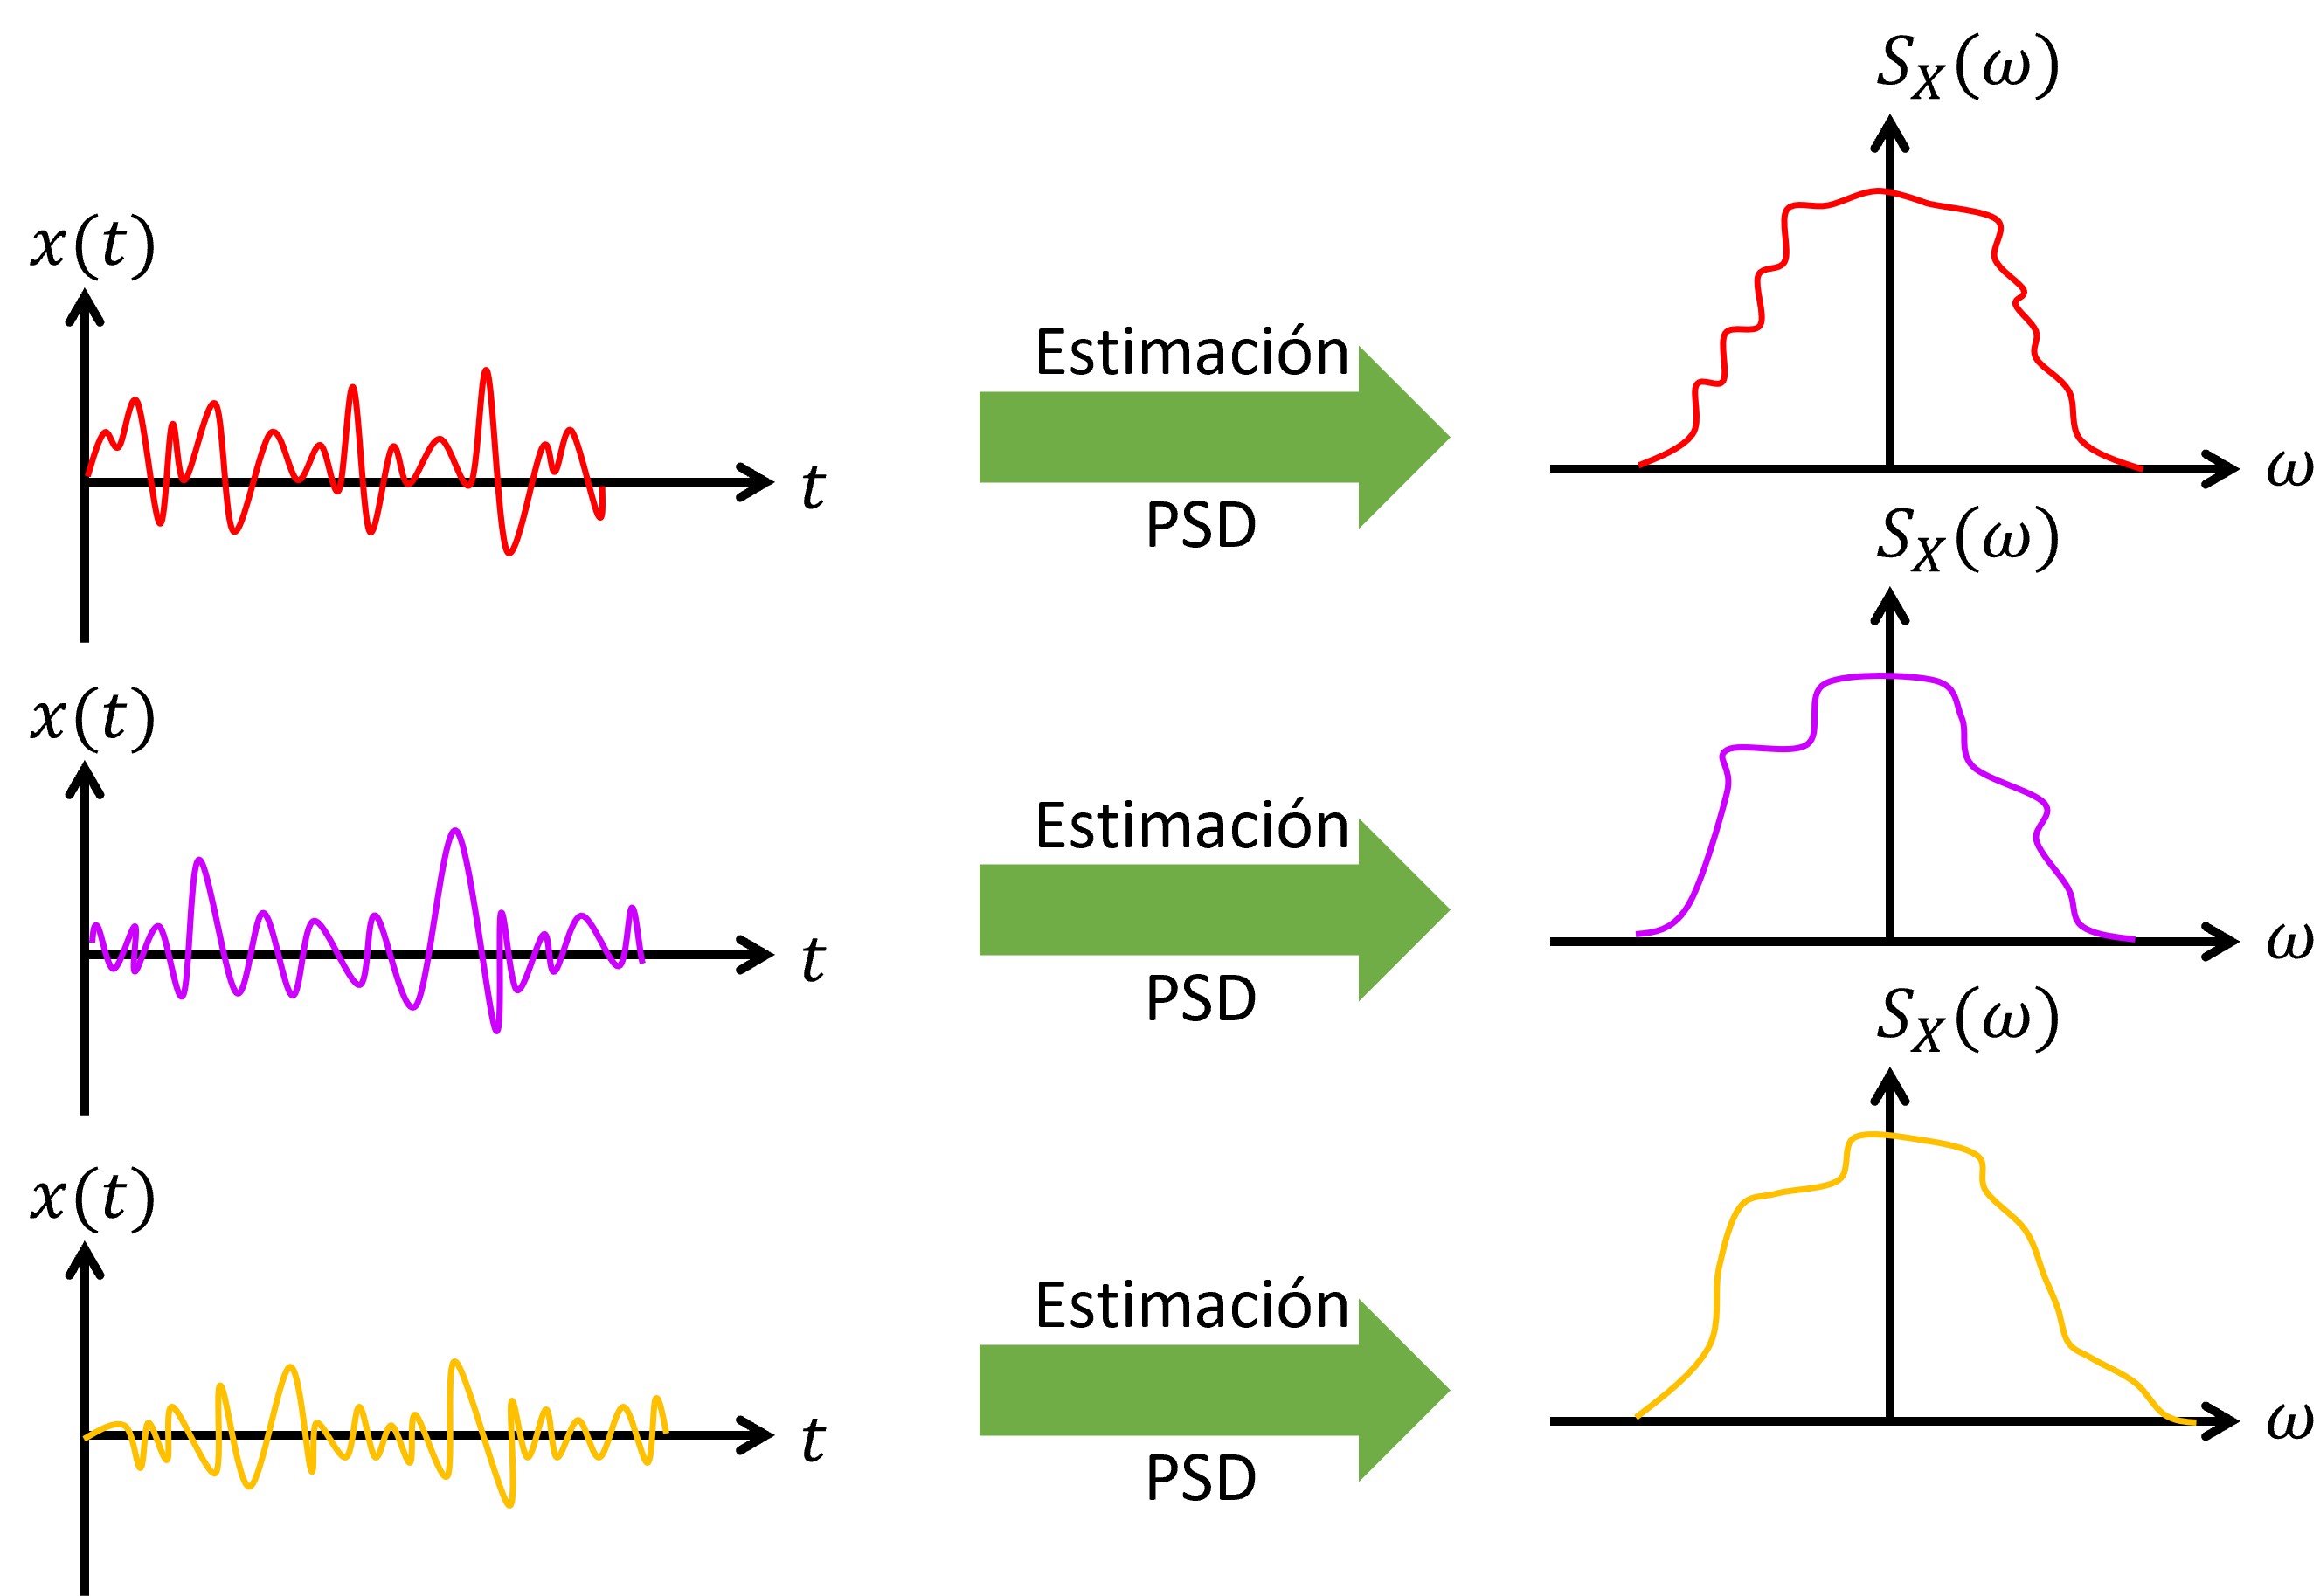
\includegraphics[scale=0.6]{Figuras/PSD_realizaciones.png}
    \end{figure}
    \item Tres realizaciones de $x[k]$ nos entegan disintas estimaciones del PSD.
\end{enumerate}

Cada estimación del PSD es una realización de un proceso estocástico.\\
\par Vamos a caracterizar el PSD utilizando la media y varianza:
\begin{enumerate}
    \item Queremos que la media del PSD se acerque al valor real del PSD.
    \item Queremos que la varianza del PSD sea pequeña.
\end{enumerate}

\underline{Ejemplo}: Considere el sgte. p.e.:
\begin{align*}
    x[n]=A+\omega[n]
\end{align*}
donde $A$ es una constante y $\omega[n]$ es ruido blanco, de media cero, $\sigma^2$.\\
\par Dada una secuencia finita $\{x[0],x[1]...,x[N-1]\}$, estimar A:\\
\par Estimador razonable: $\hat{A}=\frac{1}{N}\sum_{n=0}^{N-1}x[n]$ ``media muestral de A''.\\
\par Queremos dos cosas:
\begin{enumerate}
    \item Que $\hat{A}$ converja al valor correcto de $A$: 
    $$\mathbb{E}\{\hat{A}\}=A \quad \text{ estimador es insesgado}$$
    Sino, $\hat{A}$ es sesgado. Si no se cumple, pero $$lim_{N\to\infty} \mathbb{E}\{\hat{A}\}=A \quad \text{estimador asintóticamente insesgado} $$
    \item La varianza de $\hat{A}$ sea pequeña
    $$\text{var}\{\hat{A}\}\to 0 \quad \text{quizás aumentando N se disminuye la dispersión de }\hat{A}$$
\end{enumerate}

\underline{Objetivos}: Estimar $\hat{S}_x(\omega)$ tal que:
$$\mathbb{E}\{\hat{S}_x(\omega)=S_x(\omega) $$ y 
$$\text{var}\{\hat{S}_x(\omega)\}=\text{pequeño} $$ 

\section{Periodograma}
\underline{Definición}: 
\begin{align*}
    \hat{S}_{PER}[k] =\frac{1}{N}\bigg|\sum_{n=0}^{N-1}x[n]e^{-j2\pi nk/N}\bigg|^2
\end{align*}

\underline{Nota}: 
\begin{enumerate}
    \item Considera el cálculo del DFT en vez de TF contínua
    \item Considera un estimador neutral para el cálculo de la $\mathbb{E}\{\cdot \}$
\end{enumerate}

Ahora, hay que preguntarse:
\begin{enumerate}
    \item ¿Es $\hat{S}_{PER}[k]$ insesgado? 
    \item ¿$\text{var}\{\hat{S}_{PER}[k]\}$ es pequeña? 
\end{enumerate}

\underline{Respuestas}:
\begin{enumerate}
    \item $\hat{S}_{PER}[k]$ es sesgado, pero es asintóticamente insesgado
    $$ \lim_{N\to\infty}\mathbb{E}\{\hat{S}_{PER}[k]\}=S_x[k]\}$$
    \item Varianza de $\hat{S}_{PER}[k]$ no tiende a cero para $N\to \infty$ $\Longrightarrow$ Problema
    
    $$\text{var}\{\hat{S}_x(\omega)\}=\sigma^4 $$ 
\end{enumerate}

donde $\sigma^2=S(\omega)$ si $x[n]$ es un ruido blanco.\\
\par Principales problemas del periodograma:

\begin{enumerate}
    \item Estimación sesgada
    \item Varianza no decrece con aumento $N$
    \item Fluctuaciones rápidas
    \begin{figure}[H]
    \centering
    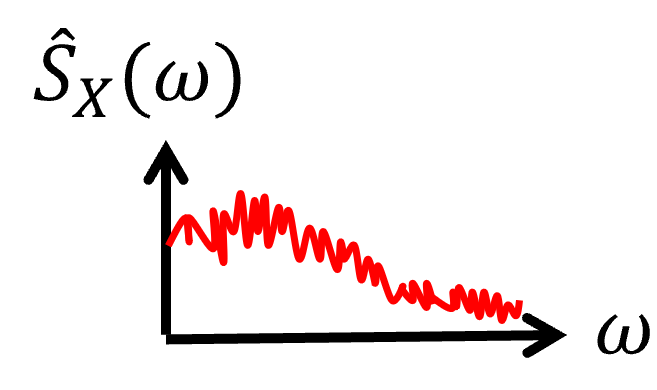
\includegraphics[scale=0.7]{Figuras/fluct.png}
    \end{figure}
\end{enumerate}

\subsection{Periodograma Modificado}
Métodos que modifican el periodograma clásico, para resolver los problemas estacionarios:
\begin{enumerate}
    \item Periodograma modificada (uso de ventanas)
    $$\hat{S}_{MP}(\omega)=\frac{1}{N\cdot U}\bigg| \sum_{n=0}^{N-1} x[n]\omega[n]e^{-j\omega n} \bigg| ^2 $$
    donde $\omega[n]$: ventana en el dominio del tiempo.
    $$U=\frac{1}{N}\sum_{n=0}^{N-1}|\omega[n]|^2 \quad \text{: factor de escala}$$
    
    \item Método de Bartlett (promedio de periodogramas)
    \begin{figure}[H]
    \centering
    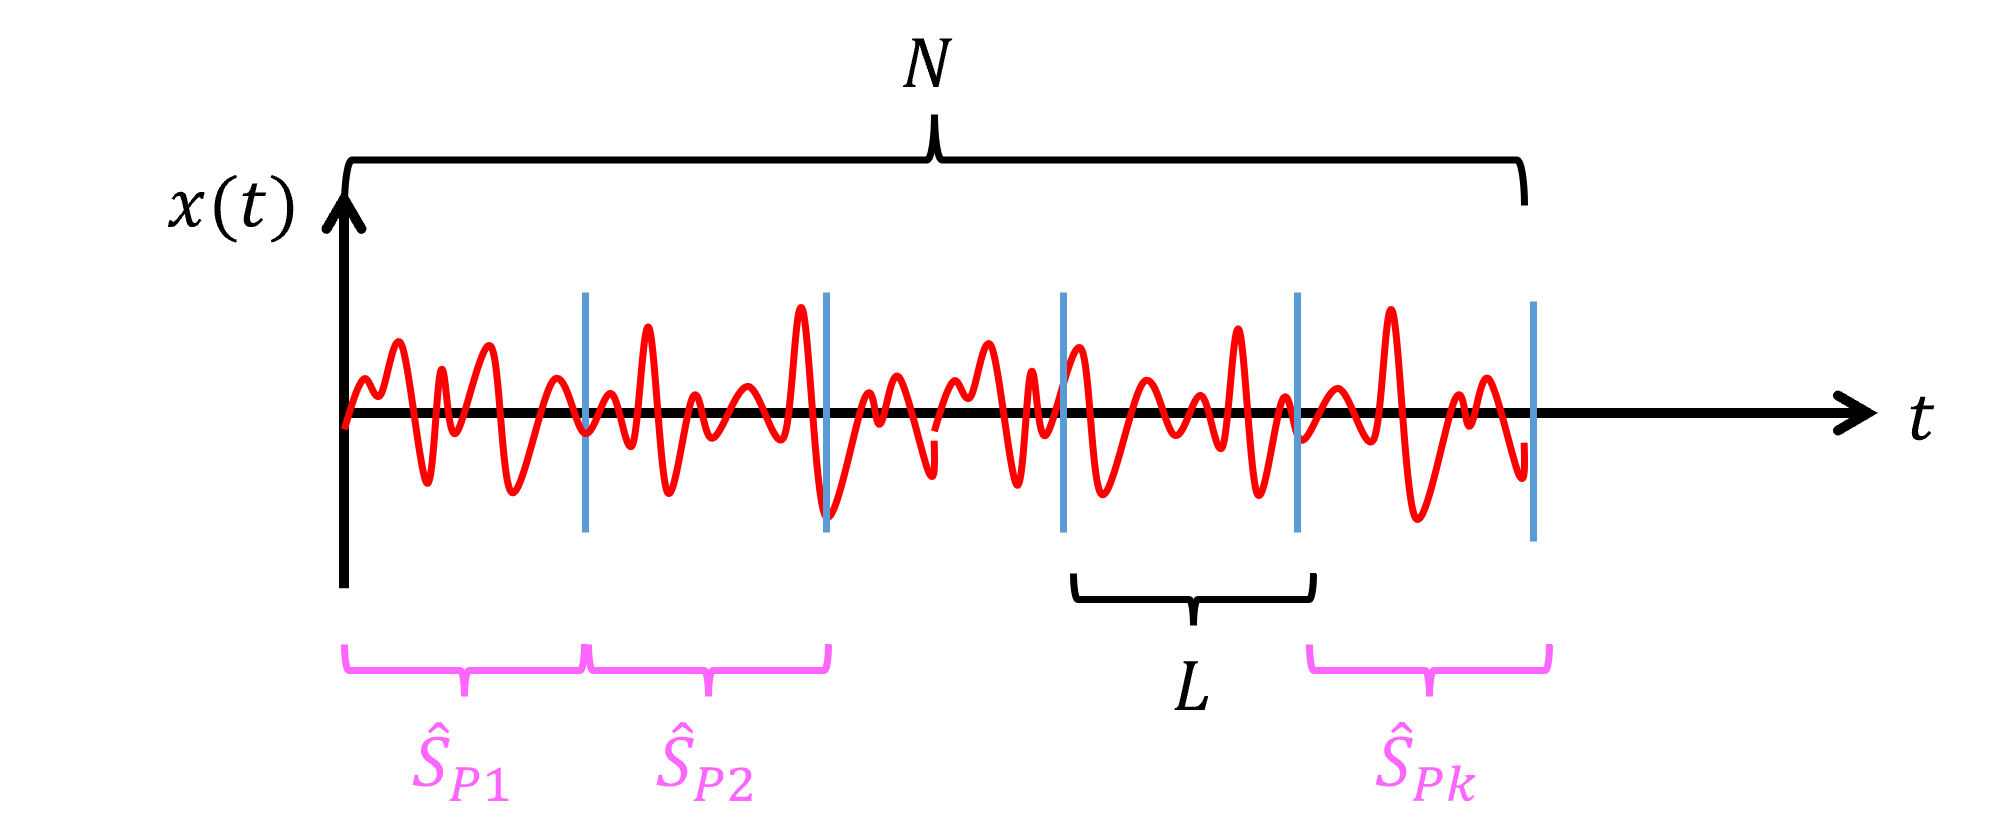
\includegraphics[scale=0.7]{Figuras/ventana1.png}
    \end{figure}
    $$\hat{S}_B(\omega)=\frac{1}{K}\sum_{i=0}^{K-1}\Bigl\{\frac{1}{L}\bigg|\sum_{n=0}^{L-1}x_i[n]e^{-j\omega n} \bigg|^2 \Bigr\} $$
    donde: \begin{itemize}
        \item i: bloque ``i'' de longitud L
        \item K: cantidad de bloques
        \item L: tamaño del bloque
    \end{itemize}
    $$\Longrightarrow  \text{var}\{\hat{S}_X(\omega)\} \approx \frac{1}{K}S_X^2(\omega)$$
    
    
    Problemas:
    \begin{itemize}
        \item Más bloques $\Longrightarrow$ bloques más cortos
        \item Blques cortos $\Longrightarrow$ peor resolución en frecuencia, $\Delta \omega$ es grande.
    \end{itemize}
    $$X[k] = \sum_{n=0}^{L-1}x[n]e^{-j2\pi nk/L} \quad \text{(DFT)}$$
    $\Longrightarrow$ ``Trade-off'': Varianza vs resolución.
    
    \item Método de Welch (promedio de periodogramas con ventanas)
    \begin{figure}[H]
    \centering
    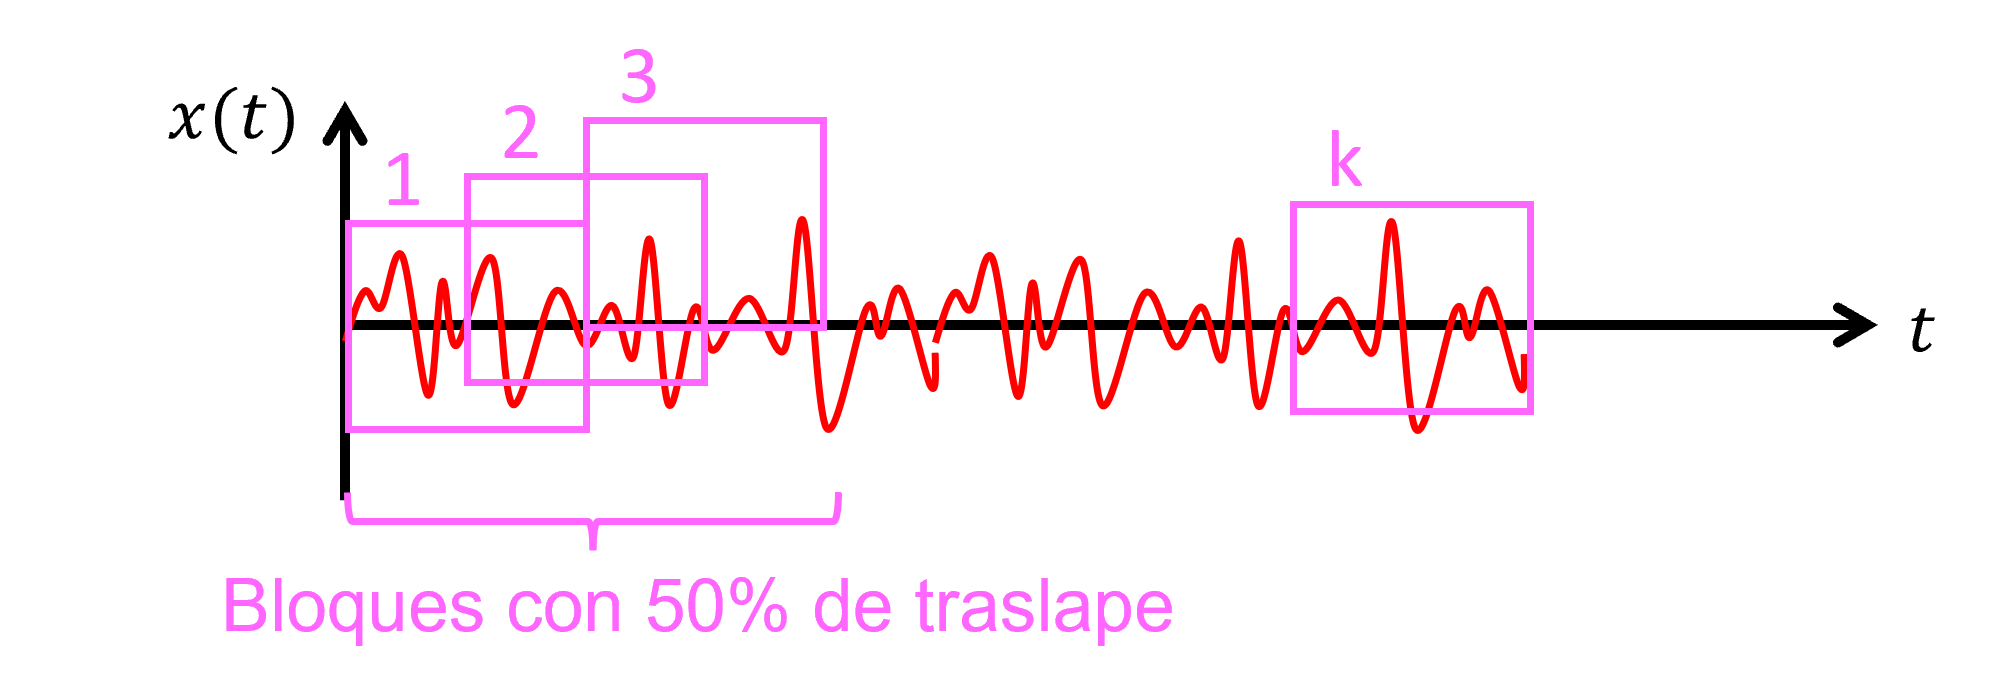
\includegraphics[scale=0.7]{Figuras/ventana2.png}
    \end{figure}
    $$\hat{S}_W(\omega) =\frac{1}{KLU}\sum_{i=0}^{K-1}\bigg| \sum_{n=0}^{L-1} x_i[n]\omega[n]e^{-j\omega n} \bigg|^2$$
    $$\text{var}\{\hat{S}_W(\omega)\} \approx \frac{9}{16}\frac{L}{N}S_x^2(\omega) $$
    Recomendación: En Matlab: \texttt{cpsd()}: cross power spectral density (método de Welch)
    
    \item Método de Blackman-Tucky
    
    
\end{enumerate}